\documentclass{template/socthesis}

\usepackage{subcaption}
\usepackage{amsmath}
\usepackage{enumitem}
\usepackage{hyperref}
\usepackage{gensymb} % balíček symbolů
\usepackage{booktabs}

\usepackage[toc,page]{appendix}
\usepackage{color} % balíček pro obarvování textů
\usepackage{xcolor}  % zapne možnost používání barev, mj. pro \definecolor
\definecolor{mygreen}{RGB}{0,150,0} % nastavení barev odkazů 
\usepackage{listings} % balíček pro formátování zdrojových kódů 
\usepackage[author=,status=draft]{fixme} % vkládání poznámek  
% dva módy (status): draft (poznámky se zobrazují v PDF) / final (poznámky se nezobrazují v PDF)
\usepackage{multirow}

\lstset { %
    language=C++,
    backgroundcolor=\color{black!5}, % set backgroundcolor
    basicstyle=\footnotesize,% basic font setting
}

\hyphenation{PROTOPlant}

\addbibresource{text.bib}
\nocite{*}

\titlecz{Automatický skleník}
\titleen{Automatic greenhouse}
\author{Petr Štourač}
\field{7}
\school{Střední průmyslová škola a~Vyšší odborná škola Brno, Sokolská, příspěvková organizace}
\mentor{Mgr. Miroslav Burda}
\mentorstatement{Mgr. Miroslava Burdy}

% Změňte, pokud se liší
%\region{Jihomoravský}
\placefooter{Brno 2020}


%\usepackage{hyperref} % balíček pro hypertextové odkazy
% \url{www.odkaz.cz}
% \href{http://www.odkaz.cz}{Text který bude jako odkaz}
% \hyperlink{label}{proklikávací_text} - odkaz na text 
% \hypertarget{label}{cíl_odkazu} - cíl odkazu 
 

\begin{document}

\maketitle

\makecopyrightstatement{V~Brně}

\makethanks{Děkuji svému školiteli Mgr. Miroslavu Burdovi za obětavou pomoc, podnětné připomínky a~hlavně nekonečnou trpělivost, kterou mi během práce poskytoval. Dále děkuji Kateřině Jelínkové za kontrolu gramatické správnosti a~korekce anglických textů. Kromě toho děkuji vyučujícím na naší škole za jejich podporu. Poděkování patří i Robotárně -- pobočce DDM Helceletova Brno za možnost využívání jejích prostor a vybavení k práci na SOČ.}

\pagestyle{empty}

\section*{Anotace}
Zahradničení je dnes naprosto běžnou zájmovou činností. Mnoho lidí mající takovou zálibu je ovšem velmi časově vytížených. Kromě práce se musí starat mnohdy i o~rodinu a~na péči o~rostliny jim často jednoduše nezbývá čas. Jedním z~těchto lidí je i můj táta, který mě inspiroval k~vytvoření PROTOPlantu -- systému pro snadnou a~levnou automatizaci skleníku. 

Cílem práce je vytvořit univerzální a~dostupný systém pro automatizaci skleníku, který by usnadnil péči o~rostliny časově vytíženým lidem. 

\subsection*{Klíčová slova}
automatizace skleníku, ESP32, PROTOPlant, automatizace, open-source hardware, open-source software

\vspace{20mm}

\section*{Annotation}
Gardening is a~very common hobby today. However, many people who likes this activity doesn't have enough time for it. 
Beside work, they have to take care of their families and after this, they don't have any time to take care of plants. 
My dad is exactly this kind of man. 
And that inspired me to create PROTOPlant -- system for easy and cheap greenhouse automation.

Goal of this thesis is to create universal and available system for greenhouse automation, that will make it easier for these people to take care of their plants.

%\fxnote[author=PŠ]{Přeložím během dnešního večera}

\subsection*{Keywords}
greenhouse automation, ESP32, PROTOPlant, automation, open-source hardware, open-source software

\newpage
\pagestyle{plain}

\tableofcontents % vysází obsah

%%% Začátek práce
\setcounter{figure}{0}
\setcounter{table}{0}
\newpage

% Uvod prace
\chapter*{Úvod}
\addcontentsline{toc}{chapter}{Úvod}

Zahradničení je dnes naprosto běžnou zájmovou činností. Mnoho lidí majících takovou zálibu je ovšem velmi časově vytížených. Kromě práce se musí starat mnohdy i o~rodinu a na péči o~rostliny jim často jednoduše nezbývá čas. Jedním z~těchto lidí je i můj táta, který mě inspiroval k~vytvoření PROTOPlantu - systému pro snadnou a levnou automatizaci skleníku.

Cílem této práce je vytvořit univerzální a dostupný systém pro automatizaci skleníku, který by usnadnil péči o~rostliny časově vytíženým lidem. 

Systémy pro takovouto automatizaci dnes existují, jsou ovšem určené primárně pro velkozemědělství, nikoli pro člověka, který ve skleníku pěstuje několik druhů zeleniny pro sebe proto, aby ji nemusel kupovat v~obchodě, nebo který vlastní menší skleník s~okrasnými rostlinami. 

Samozřejmě, na internetu existuje spousta návodů, jak si nějaký takový „systém“ vyrobit za pomoci Arduina, nepájivého pole a pár drátků.
Takové řešení se mi ovšem nezdá příliš univerzální a pracující lidé nemají mnohdy čas si takto hrát.
Zároveň pro sestavení něčeho takovového potřebují mít určité znalosti v~elektrotechnice.

Kromě toho jsem chtěl, aby bylo možno systém v~budoucnu připojit k~internetu a sledovat jej tak například z~dovolené, případně měnit nastavení.

Při vytváření práce jsem si dal za cíl, aby byl systém:
\begin{itemize}
    \item kompletně open-source
    \item levný
    \item modulární
    \item snadný na ovládání
    \item univerzální
\end{itemize}

Dalším z~cílů tohoto projektu je úspora energií (elektřina, voda), které lze díky automatizaci dosáhnout.
V~průběhu práce jsem systém nazval \B{PROTOPlant}.

\newpage


% Motivace
\chapter{Motivace}
Jak již zmiňuji v~úvodu, k~nápadu vytvořit PROTOPlant mě dovedl můj otec, který má zálibu v~pěs\-to\-vá\-ní orchidejí.
Má na ně i velký skleník, na který ovšem z~pracovních důvodů nemá příliš času.
Napadlo mne tedy, že je jistě mnoho dalších lidí, kteří jsou na tom s~časem velmi podobně, jako můj otec.

Nejdříve jsem přemýšlel pouze nad regulací teploty otevíráním oken.
Později přibylo i zavlažování a~nakonec jsem se rozhodl, že z~tohoto nápadu udělám komplexní systém i s~připojením k~internetu.
Díky tomu by bylo možné sledovat stav skleníku, nebo měnit nastavení systému jednoduše přes web, nebo mobilní aplikaci například z~práce, nebo z~dovolené. 

V~minulém roce jsem na systému začal pracovat intenzivně a~účastnil se s~ním i loňského ročníku SOČ, kde jsem na celostátní přehlídce dosáhl na šesté místo v~oboru Elektrotechnika.
To mě motivovalo na něm dále pracovat a~rozvíjet jej.

\fxnote[author=PŠ]{\textcolor{mygreen}{Zde je ještě potřeba provést úpravy.}}

\newpage

% Kapitola zabyvajici se konkurenci
\chapter{Konkurence}

\newpage

% Popis funkci, aneb „Co to vsechno umi?"
\chapter{Funkce PROTOPlantu, aneb „Co to všechno umí?“}
V~této kapitole se pokusím rozebrat funkce řídící jednotky a~dalších přídavných modulů.
Jednotlivé funkce jsou přehledně vyobrazeny na schématech \ref{fig:FEATURES_WHOLE_SMALL} a~\ref{fig:add-MODULES}.
Mezi nejdůležitější funkce PROTOPlantu patří:
\begin{itemize}
    \item možnost řízení ventilace pomocí otevírání oken, nebo ventilátorů
    \item řízení zavlažování
    \item měření teploty a~vlhkosti vzduchu
    \item měření vlhkosti půdy
    \item možnost vytápění
    \item podpora Wi-Fi -- možnost sledování stavu skleníku přes internet, nebo pomocí mobilní aplikace (funkce zatím ve vývoji)
    \item možnost přidání funkce řízení osvětlení
\end{itemize}

\fxnote[author=PŠ]{\textcolor{mygreen}{Na schématu otočit šipky u senzorů a prohodit senzory s výstupy.}}
\begin{figure}[htbp]
    \centering
    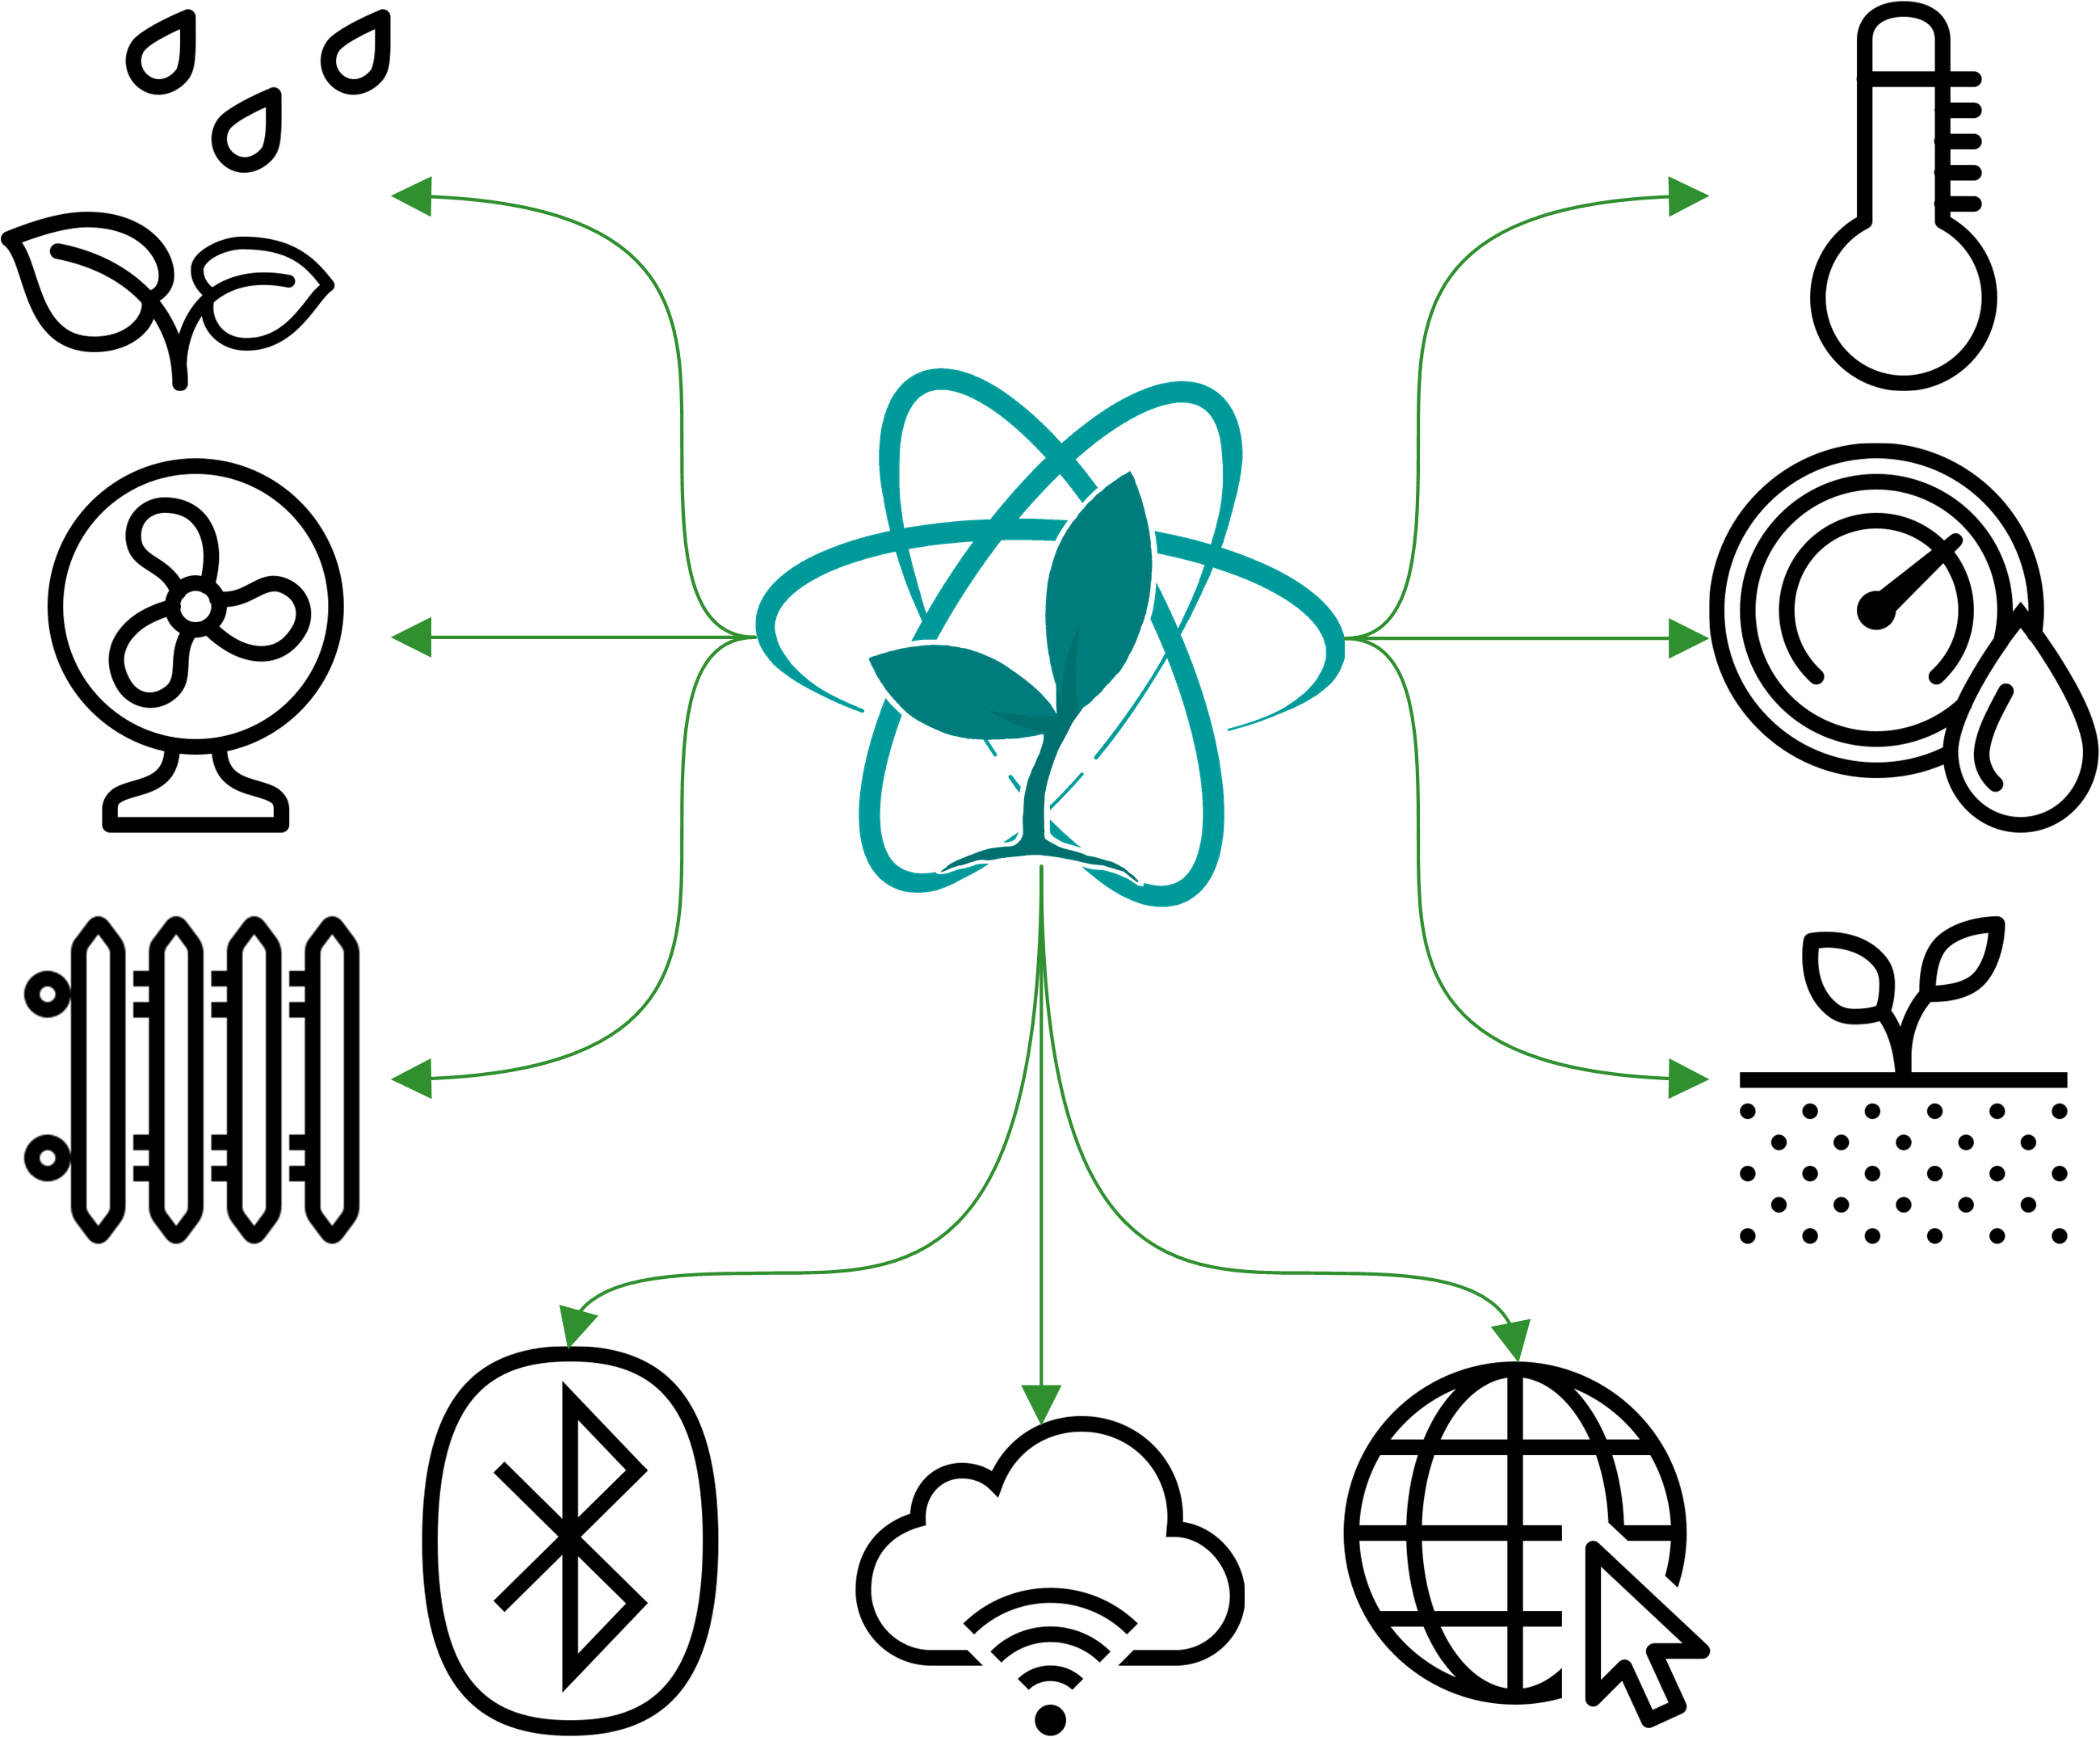
\includegraphics[scale=0.7]{img/FUNCTIONS/PROTOPLANT_FC.png}
    \caption{Zjednodušený diagram funkcí PROTOPlantu.}
    \label{fig:FEATURES_WHOLE_SMALL}
\end{figure}

\section{Funkce řídící jednotky}
Řídící jednotka, neboli PPCU je zároveň i základním modulem celého systému.
Sama o~sobě je schopna vykonávat spoustu funkcí.
Její schopnosti se pak dají ještě více rozšířit dalšími moduly.
Mezi nejdůležitější funkce patří:
\begin{itemize}
    \item dva víceúčelové výstupy pro připojení např. čerpadel, aktuátorů ovláda\-jí\-cích okna, ventilátorů a~jiných spotřebičů
    \item možnost připojení až 30-ti senzorů pro měření teploty (viz kapitola \ref{sec:DS18B20})
    \item 6 volných víceúčelových pinů pro připojení jakýchkoliv dalších periferií (senzory půdní vlhkosti, řízení osvětlení atp.)
    \item možnost připojení k~internetu
    \item LCD displej pro zobrazování naměřených hodnot
\end{itemize}

\section{Funkce dalších modulů}
Jak jsem již zmínil, s~pomocí přídavných modulů se dají funkce PPCU ještě více rozšířit.
Nutno ovšem poznamenat, že některé moduly jsou stále ve vývoji, jiné zatím ve stádiu konceptu.
\newline

\noindent\B{Modul RCM} (viz \autoref{subsec:RCM}) přidává možnost PROTOPlant vzdáleně ovládat a~měnit nastavení z~pohodlí domova.
Díky tomu není potřeba pro změnu nastavení systému opouštět obývací pokoj a~chodit do skleníku. \newline

\noindent\B{Modul PCM} (viz \autoref{subsec:PCM}) je určen pro přidání dalších výstupů pro připojení čerpadel.
Díky tomu je možno zavlažovat každou část skleníku nezávisle na sobě použitím samostatných čerpadel. 
Zároveň je díky němu možno kontrolovat hladinu vody v~nádrži (pokud tedy skleník nějakou má).\newline

\noindent\B{Modul SEM} (viz \autoref{subsec:SEM}) slouží k~připojení dalších senzorů, respektive rozšíření pokrytí senzorikou ve větších sklenících.
V~menších sklenících je PPCU schopna svojí senzorikou dostatečně pokrýt celý prostor.\newline

\noindent\B{Modul SHSM} (viz \autoref{subsec:SHSM}) přidává možnost připojení senzorů pro měření vlhkosti půdy na několika místech současně.\newline

\newpage

% Jednotlive moduly PROTOPlantu
\chapter{Jednotlivé moduly PROTOPlantu}
PROTOPlant je modulární systém - není tedy jedním velkým celkem se všemi funkcemi přímo zaintegrovanými.
V~této kapitole se zaměřím na podrobný popis jednotlivých modulů.

\section{Řídící jednotka (PPCU)}
PPCU, neboli řídící jednotka je hlavním modulem celého systému.
Samotné PPCU tvoří elektroinstalační box s~krytím IP65.
Na přední části se nachází ovládací panel s~LCD displejem a ovládacími tlačítky.
Z~bočních stran jsou instalovány vodotěsné průchodky pro provlečení kabelů.

Uvnitř se nachází základní deska (viz \autoref{subsec:motherBoard}) a zdroj napájení.

\section{Přídavné moduly PROTOPlantu}
Kromě samotné řídící elektroniky je možno PROTOPlant rozšířit i o~přídavné moduly. 
Na vývoji těchto modulů se zatím stále pracuje.
Těchto modulů existuje hned několik:

\begin{itemize}
    \item Komunikační a napájecí modul (CIPM - Communication Interface and Power Module -- modul potřebný pro drátové připojení ostatních modulů, viz \autoref{subsec:CIPM})
    \item Napájecí rozdělovač (PSpl - Power Splitter)
    \item Modul určený pro měření půdní vlhkosti (SHSM - Soil Humidity Sensorics Module -- modul vybavený senzory pro měření vlhkosti půdy, viz \autoref{subsec:SHSM})
    \item Modul rozšíření pokrytí senzorikou (SEM - Sensorics Expansion Module -- modul pro zvýšení počtu senzorů připojených k~PROTOPlantu, viz \autoref{subsec:SEM})
    \item Modul ovládání čerpadel (PCM - Pump Control Module -- modul pro sledování hladiny vody v~nádrži a ovládání čerpadla, viz \autoref{subsec:PCM})
    \item Modul vzdáleného ovládání (RCM - Remote Control Module -- modul pro připojení vzdáleného ovládacího panelu, viz \autoref{subsec:RCM})
\end{itemize}
Zjednodušené schéma zapojení a funkce jednotlivých modulů naleznete na \autoref{fig:add-MODULES}.

\paragraph{Napájení přídavných modulů}
je prováděno ve čtyřech režimech.
\begin{itemize}
    \item napájení přímo z~řídící jednotky
    \item napájení z~externího zdroje přes CIPM
    \item napájení přes PSpl
    \item napájení každého modulu odděleně
\end{itemize}

\subparagraph{Napájení přimo z~řídící jednotky}
je možno použít pouze tehdy, když je připojen maximálně jeden modul a to z~důvodu, aby bylo zabráněno podpětí celého systému.
Modul je takto připojen přímo k~napájecímu okruhu A~řídící jednotky (viz \autoref{par:PowerCircuitA}).

\subparagraph{Použití externího zdroje připojeného k~CIPM}
\label{subpar:suplyingViaCIPM}
je použitelné v~případě, kdy uživatel upřednostňuje kabelovou komunikaci mezi moduly a řídící jednotkou.
Při napájení v~tomto režimu je počet připojitelných modulů omezen pouze výkonem zdroje napájení připojeného k~CIPM.
Na vstupní napájecí svorkovnici je připojen externí zdroj. 
Kromě dvou kabelů pro komunikaci jsou na výstupu připojeny i napájecí kabely od jednotlivých modulů.

\subparagraph{Napájení přes PSpl}
funguje na velmi podobném principu, jako předchozí varianta. 
K~PSpl je na vstupní svorkovnici připojen externí zdroj napájení.
Na výstupních svorkovnicích jsou připojeny napájecí kabely jednotlivých modulů.
Tato metoda je určena primárně pro bezdrátovou komunikaci mezi řídící jednotkou a moduly.

\subparagraph{Napájení každého modulu odděleně}
je nejjednodušší metoda napájení.
Každý z~modulů je připojen vlastním kabelem přímo k~napájecímu zdroji.
Primárně je určena pro bezdrátovou komunikaci mezi jednotlivými moduly. 

\subsection{Komunikační a napájecí modul - CIPM}
\label{subsec:CIPM}
Tento modul funguje jako propojovací uzel mezi řídící jednotkou a všemi přídavnými moduly.
Dále slouží pro připojení externího napájení pro jednotlivé další moduly (viz \autoref{subpar:suplyingViaCIPM}).

\subsection{Modul měření vlhkosti půdy - SHSM}
\label{subsec:SHSM}
Modul určený pro připojení senzorů měřících vlhkost půdy.
Tento modul je zatím stále ve stádiu konceptu.

\subsection{Modul rozšíření senzoriky - SEM}
\label{subsec:SEM}
Modul určený pro zvýšení pokrytí prostoru skleníku přidáním dalších enviromentálních senzorů.
Pro malé, případně středně velké skleníky není tento modul potřebný. 
Ve velkých sklenících již své uplatnění najde vzhledem k~tomu, že je vybaven vlastní řídící elektronikou a jediným omezením je dosah zvoleného způsobu komunikace s~řídící jednotkou.

\subsection{Modul řízení čerpadel - PCM}
\label{subsec:PCM}
Valná většina zahrádkářů má pro svůj skleník i nádrž na vodu.
Tento modul je určen pro sledování hladiny vody v~ní a případné spínání čerpadla, které má za úkol v~nádrži vodu doplňovat.

\subsection{Modul vzdáleného ovládání - RCM}
\label{subsec:RCM}
Byl vytvořen pro zjednodušení nastavení a ovládání PROTOPlantu.
Skládá se ze dvou částí. 
Komunikační části, kterou lze připojit k~základní desce PROTOPlantu a ovládacího panelu. 
Uživatel ovládací panel nainstaluje na zeď přímo v~domě a může díky němu vzdáleně ovládat celýPROTOPlant přímo z~pohodlí domova. 

\subsection{Uložení řídící elektroniky}
Řídící elektronika (základní deska, řadiče, kabeláž atp.) je uložena v~průmyslových elektroinstalačních boxech s~krytím IP65 (\It{úplná prachotěsnost a odolnost proti tryskající vodě} \cite{IP_ratings}).
Vyvedení kabelů z~těchto boxů je řešeno s~pomocí kabelových průchodek se stejnou úrovní krytí.

Upevnění řídící elektroniky do těchto boxů je řešena díly vytisknutými na 3D tiskárně z~materiálu PET-G.
Ten jsem zvolil pro jeho odolnost a nehygrofilnost.

Konstrukci pro upevnění tvoří zpravidla 2 části:
\begin{itemize}
    \item montážní deska
    \item kabelový unašeč
\end{itemize}

\noindent\B{Montážní deska} je největší částí celého držáku. 
Na spodní straně se nachází drážky pro správné umístění do boxu.
Z~jedné z~bočních stran se nachází drážky pro umístění kartuše se silikagelem.
Ze strany směřující do volného prostoru boxu se nacházejí výstupky, které se zasunou do drážek v~montážní desce pro zdroj.
Na horní straně jsou umístěny otvory pro připevnění základní desky a drážky pro upevnění kabelových unašečů.

\noindent\B{Kabelové unašeče} jsou částí složenou z~více menších dílů.
Jejich úkolem je upevnění kabelů do větších svazků pro vyšší přehlednost.

%\section{Ochrana elektroniky před přehřátím a vlhkostí}
%To be done.

\newpage

% Prubeh vyvoje ProtoPlantu
\chapter{Průběh vývoje ProtoPlantu}
Za dobu vývoje ProtoPlant prošel můj systém spoustou velkých změn.
Vývoj byl započat začátkem roku 2018.
Za tu dobu vyšlo již několik verzí softwaru i hardwaru.

\section{ProtoPlant x1.0 až x4.0 (tzv. legacy verze)}
Původní verze ProtoPlantu byly celkem 4 stabilní a několik vývojových.
Tyto 4 stabilní verze jsou ve zkratce popsány níže.

\subsection{Verze x1.0}
Nejstarší funkční verze ProtoPlantu, založená na Arduinu DUE. 
Jeho software tvořilo jedno, stále se opakující vlákno.
Nevýhodou tohoto postupu bylo nepřesné časování některých úkonů způsobeném používáním blokujících operací.
Tato verze byla pouze shluk kabelů, přes které byly k Arduinu připojeny jednotlivé moduly senzorů.
Byla schopna pouze měřit teplotu a s pomocí relátek ovládat aktuátory, které následně otevíraly, nebo zavíraly okna.
Inverze polarity napájení byla řešena použitím třech relé.
Dvou, která křížově spínala kladný pól napájení aktuátorů a třetího, který připojoval zemnící vodič.
Toto zapojení nebylo zcela ideální, vzhledem k nutnosti použití tří relé a tedy i velkému úbytku napětí.
Použité Arduino bohužel další vývoj nepřežilo.

\subsection{Verze x2.0}
Největší změnou oproti předchozí verzi byl přechod z Arduina na ESP32 devkitC.
Software byl kompletně přepsán a blokující funkce odstraněny.
Díky tomu běžel software mnohem plynuleji.
Co se týče hardwaru, tato verze již používala první prototyp základní desky, který byl osazen na univerzálním tištěném spoji.
Zároveň jsem přidal podporu LCD znakového displaye, na který se vypisovaly naměřené hodnoty ze senzorů a různé stavové hlášky.
Během vývoje této verze jsem také systém začal nazývat ProtoPlant.

\subsection{Verze x3.0 a další}
Tato verze byla v minulém roce prezentována na okresním kole SOČ.
Kromě několika prototypů základní desky, které se při jejím vývoji vystřídaly, došlo i k mnohým změnám ve funkci celého ProtoPlantu.
Doposud používaná relé, kterými ProtoPlant spínal aktuátory, bylo nutno nahradit jiným řešením.
Důvodem k tomu byl jejich příliš velký úbytek napětí, který způsoboval podpětí celé řídící elektroniky.
Hledal jsem tedy způsob, jak vyřešit spínání aktuátorů tak, aby byl napěťový úbytek co nejmenší.
Nakonec jsem objevil H-můstky VNH2SP30. 
Ty umožňují kromě regulace výstupního napětí velmi jednoduše obracet polaritu výstupů.
Pro zjednodušení zapojení při testování jsem využíval Monster Moto Shield, na kterém jsou tato VNH osazena hned dvě.
Proto mne napadlo využít druhé VNH jako víceúčelový výstup, ke kterému lze připojit čerpadlo, elektromagnetický ventil, případně jiná zařízení.
V softwaru přibyla podpora tlačítek a menu zobrazované na LCD displeji, přes které se dalo měnit nastavení systému za chodu.
Dále jsem ProtoPlant uzavřel do průmyslového elektroinstalačního boxu s krytím IP67.
Do víka boxu jsem nainstaloval LCD displej a ovládací tlačítka.

\paragraph{Verze x3.1}
byla další ze stabilních verzí zaměřená primárně na opravu softwarových chyb.
Tuto verzi jsem v minulém roce prezentoval v krajském kole SOČ.
Menu nastavení bylo přeloženo do češtiny.

\paragraph{Verze x3.2}
byla verzí prezentovanou na loňské celostátní přehlídce.

\section{ProtoPlant verze 5.0}


\newpage

% Testovani protoplantu
\chapter{Dlouhodobé testování}


\newpage

% Uspory dosazene pouzitim protoplantu
\chapter{Úspora energií dosažená s pomocí PROTOPlantu}
To be done.

\newpage

% Dostupnost a distribuce
\chapter{Dostupnost a distribuce PROTOPlantu}
Jak popisuji v~úvodu, jedním z~cílů, který jsem si dal na začátku práce na PROTOPlantu bylo šíření pod licencí open-source.
Toto jsem dodržel. 
Celý software PROTOPlantu je šířen pod licencí MIT, ostatní části (Hardware, atd.) včetně textu této práce je poté pod CC BY-NC-SA 4.0.
Co se týče hardwaru, převzatý hardware (senzory, procesor a další moduly) je z~licence vyňat.
Člověk, který tedy elektrotechnice a programování rozumí si poté může PROTOPlant bez problému sestavit sám v~pohodlí domova.

Ovšem stále je obrovské množství lidí, kteří na sestavení PROTOPlantu nemusí mít dostatečné znalosti, nebo nemají čas si jej sestavovat.
Z~toho důvodu plánuji zahájit výrobu a distribuci mého systému jakožto hotových komponent, které stačí nainstalovat a zapojit.
Ke dni \It{20. 2. 2020} jsem ve fázi, kdy připravuji výrobní podklady jednotlivých komponent, a provádím kroky vedoucí k~založení podniku.
Již v~minulém roce jsem provedl průzkum, který ukázal, že o~PROTOPlant by skutečně byl zájem.

\section{Případové studie}
Pro názorný příklad použití PROTOPlantu uvádím konkrétní případové studie.

\subsection{Malý skleník s užitkovými rostlinami}
Zahrádkář pěstující plodiny čistě pro zásobování sebe a své rodiny čerstvou zeleninou vlastní skleník s plochou obdělávané půdy 6x3 metry.
Výška skleníku jsou přibližně dva metry, jeho objem je tedy vzhledem k tvaru skleníku \B{menší, než 36~m\superscript{3}}.
Pro dostatečné pokrytí prostoru senzorikou tedy stačí dva senzory teploty (viz kapitola \ref{sec:DS18B20}) a dva senzory vzdušné vlhkosti (viz kapitola \ref{sec:DHT22}). 
Vzhledem k obdělávané ploše, stačí použít 4 senzory půdní vlhkosti.
Zavlažování je vzhledem k pěstovaným rostlinám řešeno děrovanou hadicí položenou přímo na půdě.

\fxnote[author=PŠ]{Zde přibudou fotografie babiččina skleníku a tabulka s cenami (dnes večer to spočítám)}

\subsection{Středně velký skleník s okrasnými rostlinami}
Skleník, ve kterém PROTOPlant průběžně testuji je určen pro pěstování orchidejí. 
Jeho plocha je přibližně 10~x~4~m.
Většina rostlin je v květináčích s molitanem či substrátem zavěšena v prostoru, nebo položena na stole.
Teplotní senzory jsou zde použity 4, senzory vlhkosti 3.
Vzhledem k tomu, že většina z těchto rostlin je epifytní, nesnášejí trvale vlhkou půdu. 
Z tohoto důvodu je zavlažování řešeno rozprašovačem umístěným pod stropem skleníku a upraveným nastavením jeho spínání.
Neprobíhá tedy tak často.

\fxnote[author=PŠ]{Zde přibudou fotografie velkého testovacího skleníku a opět tabulka s cenou}

\newpage

% Zaver prace
\chapter*{Závěr}
\addcontentsline{toc}{chapter}{Závěr}

Záměrem mojí práce bylo vytvořit univerzální systém pro automatizaci skleníku, který je:
\begin{itemize}
    \item open-source
    \item levný
    \item modulární
    \item snadný na ovládání
    \item univerzální
\end{itemize}

Tento cíl se mi podařilo splnit.
Lidé, kteří mají zájem si systém vytvořit najdou veškerou dokumentaci, schémata a zdrojový kód na webu \textit{www.protoplant.cz}.

Díky SOČ jsem se naučil pracovat se softwarem pro návrh PCB Autodesk EAGLE.
Zároveň jsem vylepšil své schopnosti v programování a získal spoustu dalších zkušeností v elektrotechnice a s prací na takto komplexních projektech.

Co se týče plánů do budoucna, PROTOPlant budu dále rozvíjet.
Mezi mé plány se řadí dokončení rozpracovaných modulů a další vylepšování softwaru.
Dále bych se rád zaměřil na rozšíření PROTOPlantu o možnosti z oblasti internetu věcí.

\newpage
\newpage

\appendix
\addcontentsline{toc}{chapter}{Přílohy}

\color{mygreen}
Co přidat sem?
\begin{itemize}
    \item Fotky PROTOPlantu
    \item fotky senzorů
    \item fotky dílů z 3D tiskárny
    \item další jednoduchá "zelinářská" schémátka
    \item fotky dalších DPS
\end{itemize}

\color{black}

% Tistene spoje a elektronika
\chapter{Elektronika a~tištěné spoje}
Všechny prototypy základních desek PROTOPlantu byly založeny na univerzálních tištěných spojích. Vzhledem k~tomu, že jsem po stránce vzhledu i funkčnosti nebyl s~takovýmto provedením spokojen, rozhodl jsem se nechat vyrobit vlastní tištěné spoje pro základní desku i senzorové moduly.
Díky tomuto jsem se naučil návrhu tištěných spojů a~tvorbě výrobních podkladů v~programu Autodesk EAGLE.

\section{PPMB32 -- Základní deska}
\label{subsec:motherBoard}
Základní deska je rozdělena do několika částí. 
Vzhledem k~tomu, že umím pájet velmi dobře, rozhodl jsem se pro ruční osazení všech součástek, které byly doposud osazeny pouze na různých modulech připojených k~základní desce, včetně procesoru ESP32-WROOM32D.
Z~důvodu přehlednosti jsem desku rozdělil do několika částí:

\begin{itemize}
    \item Control (ESP32-WROOM32D a~programátor)
    \item H-power (napájecí obvod a~H-můstky)
    \item SIN (SensorIN -- piny pro připojení senzorů)
    \item POUT (PowerOUT -- výstup pro napájení dalších periferií)
    \item PanCon (PanelConnect -- piny pro připojení tlačítek a~displeje na ovládacím panelu)
    \item SelfProt (SelfProtection -- senzor teploty a~piny pro připojení vnitřního detektoru vody)
\end{itemize} 

Samotná základní deska má dvě verze. Jejich rozdíly jsou vysvětleny níže.
Obě verze desky jsou kromě sekce Control osazeny stejným hardwarem, tedy:

\begin{itemize}
    \item 2x H-můstek VNH2SP30
    \item regulátory napětí 7805CV-DG od STMicroelectronics
    \item pinheady pro připojení senzorů, ovládacího panelu a~dalších periferií
    \item svorkovnicemi pro připojení napájecích kabelů a~silových výstupů
\end{itemize}

Kromě dalších součástek je přímo na desce osazen senzor DS18B20 chránící desku před přehřátím. 
Pokud teplota základní desky překročí 50~\degree C, automaticky se přeruší veškeré operace a~systém přejde do režimu nouzového chlazení (viz kapitola \ref{paragraph:CoolingMode}).

\paragraph{PPMB32-F}
Kompletní, samostatná deska. 
Je přímo osazena procesorem ESP32-WROOM32D i programátorem CP2102N. 
Má nižší profil, tudíž je možné ji použít i v~menších prostorech.
Integrovaný programátor lze s~pomocí jumperů odpojit a~přes programovací piny připojit externí. Tuto verzi jsem nazval PPMB32-F (označení F od anglického slova Full -- kompletní).
Zároveň je optimalizovaná pro strojní osazování.

\paragraph{PPMB32-E}
Vzhledem k~tomu, že je PROTOPlant veřejně dostupný, nebyl jsem si jist, zda by kompletní osazení takto velké desky zvládl i laik. 
Napadlo mě proto vytvořit i druhou desku, na které by byly osazeny dutinkové lišty pro vsazení vývojové ESP32 DevKitC. 
Odpadla by tedy nutnost kompletně osazovat sekci Control. 
Tuto verzi jsem nazval PPMB32-E (označení E od anglického slova Easy -- jednoduchý).
Je určena primárně pro ruční osazování.

\paragraph{Sekce Control}
Jak již bylo zmíněno, tato část desky zahrnuje modul procesoru ESP32-WROOM32D a~programovací obvod. 
Ten se skládá z~převod\-ní\-ku USB-UART CP2102N, tranzistorů SS8050-G (sloužících pro reset procesoru), indikačních LED diod a~mikro USB konektoru. 
Nachází se zde i jumper pro přepínání mezi externím programátorem a~programátorem přímo na desce.

\paragraph{Sekce H-power}
V~této části desky se nacházejí H-můstky VNH2SP30 společně s~regulátory napětí 7805CV-DG (výstup 5VDC) a~LM3940IT-3.3 (výstup 3,3VDC). 
Na verzi PPMB32-F je dále osazen AMS1117-3.3 pro napájení procesoru. 

V~dolní části desky se poté nacházejí dva integrované obvody VNH2SP30, z~nichž jeden (VNH1) je určen pro ovládání aktuátorů manipulujících s~okny a~druhý 
(VNH2) má několik režimů funkce podle připojeného výstupu:
\begin{itemize}
    \item disabled (výstupy jsou deaktivovány)
    \item pump (VNH je použito pro spínání čerpadla, případně stykače řídícího čerpadlo)
    \item heating (VNH je použito pro řízení topné spirály)
\end{itemize}

Napájení desky je rozděleno do tří okruhů. 

\paragraph{Okruh A}
\label{par:PowerCircuitA}
Tento okruh je určen pro napájení řídící elektroniky.
Má celkově 3 části, oddělené s~pomocí stabilizátorů napětí.
Jejich propojení znázorňuje schéma.
Rozsah vstupního napětí pro tento okruh je 7,5~VDC až 18~VDC.

\paragraph{Okruhy V1 a~V2}
Použity pro oddělené napájení jednotlivých výstupů. 
Jejich napájecí rozsahy jsou rozepsány v~tabulce \ref{fig:powerSourceCharsVNH}.

\begin{table}[h]
    \centering
    \begin{tabular}{llll}
        \hline
        \multicolumn{1}{|l|}{\textbf{Parametr}}           & \multicolumn{1}{l|}{\textbf{Min.}} & \multicolumn{1}{l|}{\textbf{Max.}} & \multicolumn{1}{l|}{\textbf{Jednotka}} \\ \hline
        \multicolumn{1}{|l|}{Vstupní napětí}              & \multicolumn{1}{l|}{5,5}           & \multicolumn{1}{l|}{16}            & \multicolumn{1}{l|}{V}                 \\ \hline
        \multicolumn{1}{|l|}{Výstupní napětí}             & \multicolumn{1}{c|}{-}             & \multicolumn{1}{l|}{16}            & \multicolumn{1}{l|}{V}                 \\ \hline
        \multicolumn{1}{|l|}{Výstupní proud}              & \multicolumn{1}{c|}{-}             & \multicolumn{1}{l|}{30}            & \multicolumn{1}{l|}{A}                 \\ \hline
        \multicolumn{1}{|l|}{Maximální kontinuální proud} & \multicolumn{1}{c|}{-}             & \multicolumn{1}{l|}{14}            & \multicolumn{1}{l|}{A}                 \\ \hline
    \end{tabular}
    \caption{Tabulka napájecích rozsahů napájecích větví VNH1 a~VNH2}
    \label{fig:powerSourceCharsVNH}
\end{table}

\paragraph{Sekce SIN}
Sekce s~piny pro připojení jednotlivých senzorů. 
S~výjimkou ochranných rezistorů je složena pouze z~pinheadů.
Jednotlivé piny jsou pro lepší přehlednost označeny přímo na desce a~podrobněji popsány v~jejím datasheetu. 

\paragraph{Sekce POUT} 
Piny pro připojení napájení dalších periferií, modulů, či senzorů.
Je připojena k~napájecímu okruhu A.
Piny jsou rozděleny na části připojené k~subokruhům A1 a~A2 s~napětím 3,3 a~5~VDC.

\paragraph{Sekce PanCon}
Dvanáctipinový konektor PanCon slouží pro připojení kabelu od hlavního řídícího panelu. 
Samotný konektor má dva zemnící vývody, dva napájecí (1~x~5~V~a~1~x~3,3~V), dva vývody sběrnice I\textsuperscript{2}C a~6 vývodů pro připojení tlačítek a~přepínačů.
Přesnější zapojení je opět k~dispozici v~datasheetech jednotlivých desek.

\section{PPSB -- Desky se senzory teploty a~vlhkosti}
Desky osazené senzory DS18B20\cite{DS18B20} (PPSB-T) a~DHT22\cite{DHT22} (PPSB-TH).
Pro oba typy desek jsem navrhl a~s~pomocí 3D tisku vyrobil vlastní krabičky.\newline

\noindent\B{PPSB-T} -- deska osazená jedním senzorem DS18B20 \cite{DS18B20} zapojeným v~režimu parazitního napájení (viz \autoref{sec:DS18B20}).
V~něm je senzor napájen přímo ze sběrnice OneWire, stačí mu tedy pro připojení pouze dva kabely (více v~\cite{DS18B20}).
Deska má jednu vstupní a~jednu výstupní stranu, senzory se takto dají řetězit.

Vizualizaci desky naleznete na obrázku \ref{fig:PPSB-T_VISUAL}.\newline \newline

\begin{figure}[h]
    \centering
   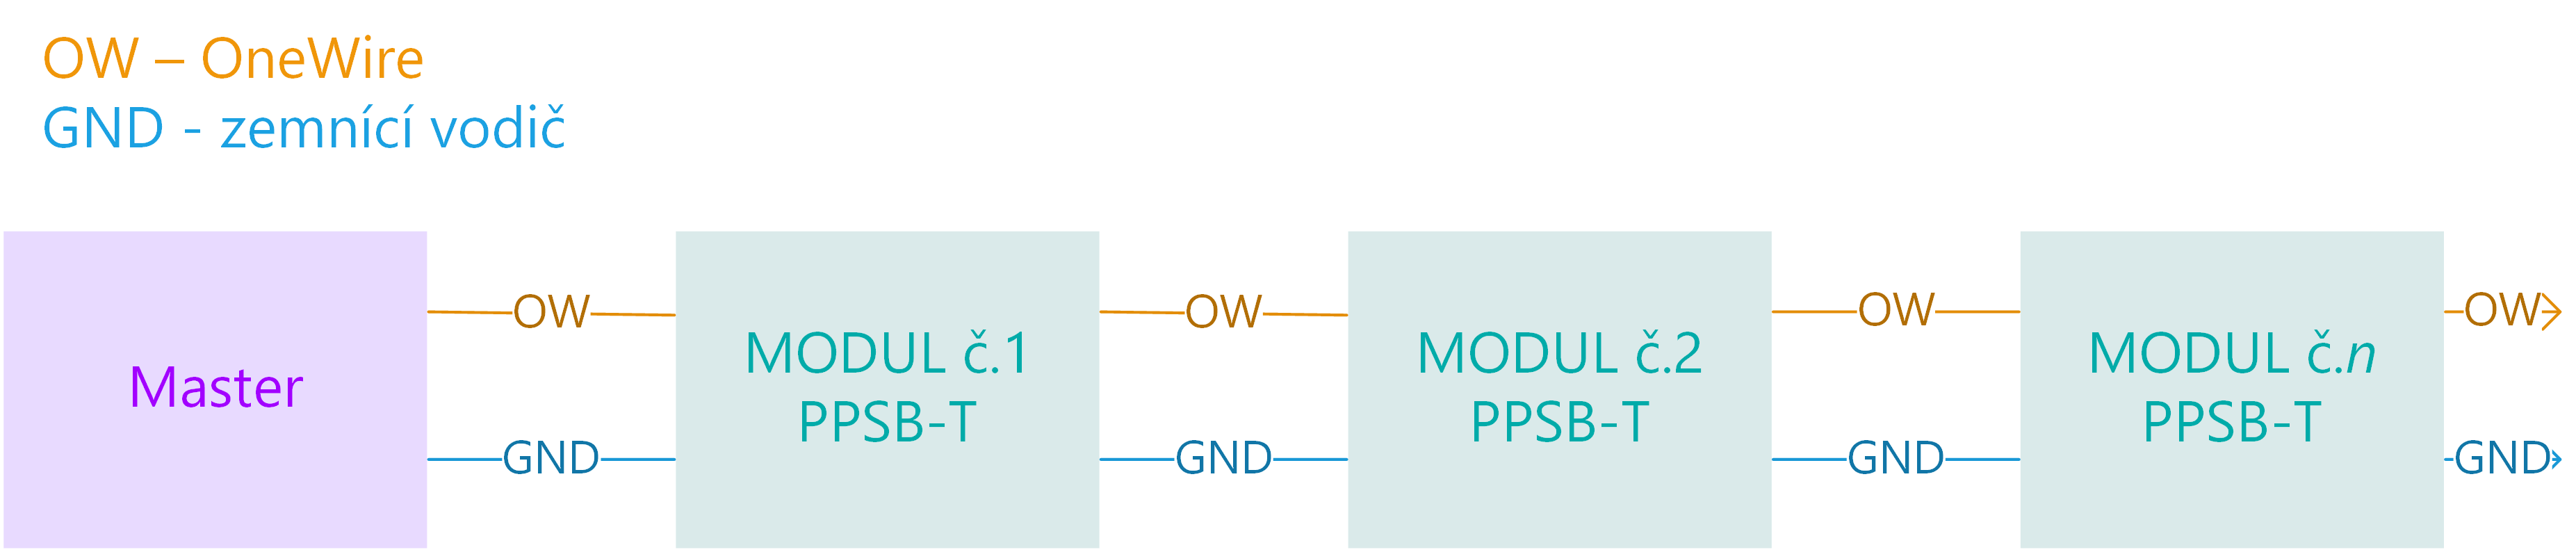
\includegraphics[width=\textwidth]{img/HARDWARE/PPSB-T_CHAIN.png}
   \caption{Řetězení desek PPSB-T.}
   \label{fig:PPSB-T_wiring}
\end{figure}

\noindent\B{PPSB-TH} osazena senzorem DHT22 \cite{DHT22} je schopna měřit vzdušnou vlhkost i teplotu.
Více o~tomto senzoru naleznete v~kapitole \ref{sec:DHT22}.
Narozdíl od PPSB-T tyto desky nelze řetězit.
Vizualizace naleznete na obrázku \ref{fig:PPSB-TH_VISUAL}.\newline

\section{Senzorika}
PROTOPlant primárně podporuje 3 typy senzorů. 
DS18B20 pro měření vzdušné teploty, DHT22 schopné měřit vlhkost i teplotu vzduchu a~senzory pro měření vlhkosti půdy.
Dále PROTOPlant podporuje připojení senzorů vlhkosti půdy pracujících na bázi elektrické vodivosti.

\subsection{DS18B20}
\label{sec:DS18B20}
Senzory určené pro měření teploty. 
Komunikují po sběrnici OneWire (více v~\cite{DS18B20}, str. 4) vytvořené společností Maxim Integrated.
Jsou určeny pro teplotní rozsahy -55~\degree C až +125~\degree C.
V~měřícím rozsahu -10~\degree C až +85~\degree C jsou schopny měřit s~přesností na $\pm0,5$~\degree C.
K~PPCU je možno připojit až 30 těchto senzorů.

%\subsection{BME280}
%\label{sec:BME280}
%To be done.

\subsection{Senzory půdní vlhkosti}
\fxnote[author=PŠ]{Dopíšu během pondělka}

\subsection{DHT22}
\label{sec:DHT22}
Čidla, která měří vzdušnou vlhkost i teplotu.
Jejich přesnost je $\pm2\%$ relativní vlhkosti a~$\pm$0,5\degree C.
Opakovatelnost měření je poté $\pm$1\% relativní vlhkosti a~$\pm$0,2\degree C.
Tyto senzory komunikují jednosběrnicově, není tedy možno je řetězit.
K~PPCU je možno připojit těchto senzorů až 6.
Více viz \cite{DHT22}.

Do budoucna zvažuji přechod na senzory AM2321 \cite{AM2321} vzhledem k~tomu, že narozdíl od DHT22 dokáží komunikovat po sběrnici I\superscript{2}C (viz kapitola \ref{sec:I2C_comm}).

\newpage

% Podrobny popis softwaru
\chapter*{Software základní desky}
\addcontentsline{toc}{chapter}{Příloha B: Software základní desky}
Tato kapitola se zaměřuje na software základní desky PROTOPlantu a detailně popisuje jeho funkci.
Na software ostatních modulů se zaměřuje následující kapitola \ref{chap:moduleSoftware}.

\paragraph{Blokové schéma funkce softwaru základní desky}
Schéma funkce softwaru základní desky je shrnuto blokovým diagramem XXX.

\section*{Sdílené knihovny}
Z~důvodu usnadnění programování základní desky i ostatních rozšiřujících modulů jsem vytvořil několik sdílených knihoven. 
V~nich je zahrnuto:
\begin{itemize}
    \item konfigurace systému
    \item nastavení jednotlivých pinů dle standardního rozložení, vč. možnosti nastavení vlastního
    \item práce s~displayem
    \item práce s~tlačítky
    \item řízení H-můstků
    \item ovládání senzorů
\end{itemize}
Díky těmto knihovnám je většina zdrojového kódu uložena v~nich. 
Koncový uživatel, který se rozhodne software modifikovat, poté pouze v~hlavním programu definuje, které moduly spustit a do konfiguračního souboru zapíše nastavení daných modulů.

\paragraph{Konfigurace softwaru}
Konfigurace softwaru pro jednotlivé verze hardwaru je řešena pomocí jednoho souboru.
Podle toho, jak jsou jednotlivá makra v~tomto souboru definována, prekompilátor následně sestaví software přímo pro danou verzi.
Část konfiguračního souboru je zobrazena níže.
V~této části lze nastavit parametry přístupového bodu Wi-Fi, který si PROTOPlant sám vytvoří, sériové linky a displeje.
\begin{lstlisting}
    //If wifi credentials not set OR wifi not found, 
    //create own AP with these credentials
    #define AP_SSID ProtoPlant
    #define AP_PASSWORD protoplant
    
    #define SERIAL_DEBUGGING    true
    #define SERIAL_BAUDRATE     115200
    
    #define DISPLAY_CONNECTED   true
    #define DISPLAY_ADDRESS     0x27
    #define DISPLAY_TIMEOUT     10000
    #define DISPLAY_COLONS      16
    #define DISPLAY_ROWS        4
\end{lstlisting}

\section*{Datové sběrnice}
PROTOPlant primárně využívá dvě datové sběrnice:
\begin{itemize}
    \item I\superscript{2}C
    \item OneWire
\end{itemize}

\noindent\B{Sběrnici I\superscript{2}C} používá PROTOPlant pro komunikaci se zařízeními na stejné desce, případně pro řízení LCD displeje instalovaného na řídícím panelu (připojení přes PanCon). 

\subparagraph{Princip}
Na sběrnici je připojeno jedno zařízení jakožto master (řídící) a jedno či více zařízení jako slave (řízená).
Tato zařízení jsou navzájem propojena dvěma dráty (proto se I\superscript{2}C někdy přezdívá TwoWire), serial clock (SCL) a serial data (SDA).
Každé ze slave zařízení má sedmibitovou adresu (např. 0xE0), která musí být pro každé zařízení na jedné sběrnici odlišná.
Některá zařízení mají tuto adresu pevně zapsanou a nelze ji měnit, zatímco u~jiných ji lze změnit.
Zařízení připojené jako v~režimu master tuto adresu nepotřebuje, vzhledem k~tomu, že on sám vždy adresuje jen jedno ze zařízení.

\subparagraph{Komunikační protokol}
Za klidového stavu (neprobíhá žádná komunikace) jsou obě linky (SDA i SCL) připojeny nastaveny na HIGH.
Jakmile chce master zahájit komunikaci, vyšle takzvaný startovní signál, po kterém následuje adresa daného zařízení, jejíž nultý bit určí, zda chce master číst, nebo zapisovat.
Dále následují datové bity.
Jakmile jsou všechna data přenesena, vyšle master stop signál, čímž ukončí komunikaci a sběrnice se vrátí do klidu.
Rychlost celého přenosu určuje pulsování linky CLK.
Celý proces názorně zobrazuje obrázek \ref{fig:I2C-protocol}.

\begin{figure}[htbp]
   \centering
   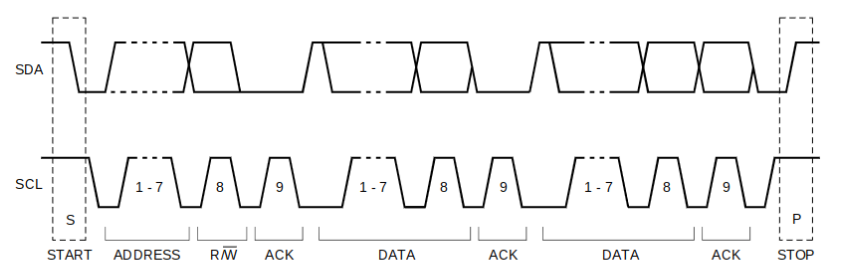
\includegraphics[width=\textwidth]{img/I2C.png}
   \caption{Celý datový přenos po I2C sběrnici. Převzato z~\cite{I2C_specs}}
   \label{fig:I2C-protocol}
\end{figure}

\paragraph{Sběrnice OneWire}
Sběrnici OneWire používá PROTOPlant pro komunikaci s~teplotními čidly DS18B20. 
Více o~této komunikační sběrnici v~\cite{DS18B20}.

\section*{Komunikace mezi řídící jednotkou a jednotlivými moduly}
PROTOPlant podporuje dva režimy komunikace řídící jednotky s přídavnými moduly:
\begin{itemize}
    \item bezdrátová komunikace přes Wi-Fi
    \item kabelová komunikace přes UART (standard RS-485)
\end{itemize}

\section*{Bezdrátová komunikace}
Je vhodná primárně pro malé skleníky v oblastech, kde nehrozí zarušení signálu.
Tento způsob komunikace je zatím stále ve vývoji.

\section*{Kabelová komunikace a RS-485}
Kabelová komunikace probíhá přes tzv. UART (Universal Asynchronnous Receiver and Transmitter - univerzální asynchronní přijímač a vysílač).
PROTOPlant využívá průmyslový standard RS-485 umožňující komunikaci s~pomocí dvojlinky.
Opět je zde uplatněn princip master - slave (řídící jednotka je master, ostatní moduly slave).
Pro tento způsob komunikace existuje několik protokolů, pro příklad velmi často používaný ModBus, nebo nedávno vytvořený JANUS\cite{JANUS}, který používám. 
Více o~principu RS-485 a samotném protokolu v~\cite[21-25]{JANUS}

\chapter*{Software dalších modulů}
\addcontentsline{toc}{chapter}{Příloha C: Software dalších modulů}

\label{chap:moduleSoftware}
Software přídavných modulů je navržen tak, aby k~jeho běhu nebyl zapotřebí velký výpočetní výkon.
Obecně lze jejich funkci znázornit blokovým diagramem \ref{fig:PPCU-to-MODULE-communication}.

\chapter*{Zvláštní stavy}
\addcontentsline{toc}{chapter}{Příloha D: Zvláštní stavy}
PROTOPlant má několik zvláštních stavů, ve kterých pracuje v omezeném režimu.
Tyto stavy slouží primárně pro zabránění poškození systému.

\paragraph{Režim nouzového chlazení}
\label{paragraph:CoolingMode}
Do tohoto režimu přejde systém v~případě, že teplotní senzor na základní desce PPCU detekuje přehřívání. 
Dojde k~automatickému vypnutí výstupů řídící jednotky.
Poté se systém restartuje, aby vyloučil chybu softwaru.
V~případě, že softwarovou chybu nedetekuje, vyčká, než se teplota sníží na běžnou provozní hodnotu, kterou průběžně vypočítává z~průměrů hodnot naměřených před prudkým nárůstem.
Po ochlazení systém pokračuje v~normálním chodu, ovšem na displeji zůstane upozornění, že k~chybě došlo.

\newpage

% Prilohy
\chapter{Obrazové přílohy}

\begin{figure}[h]
    \centering
    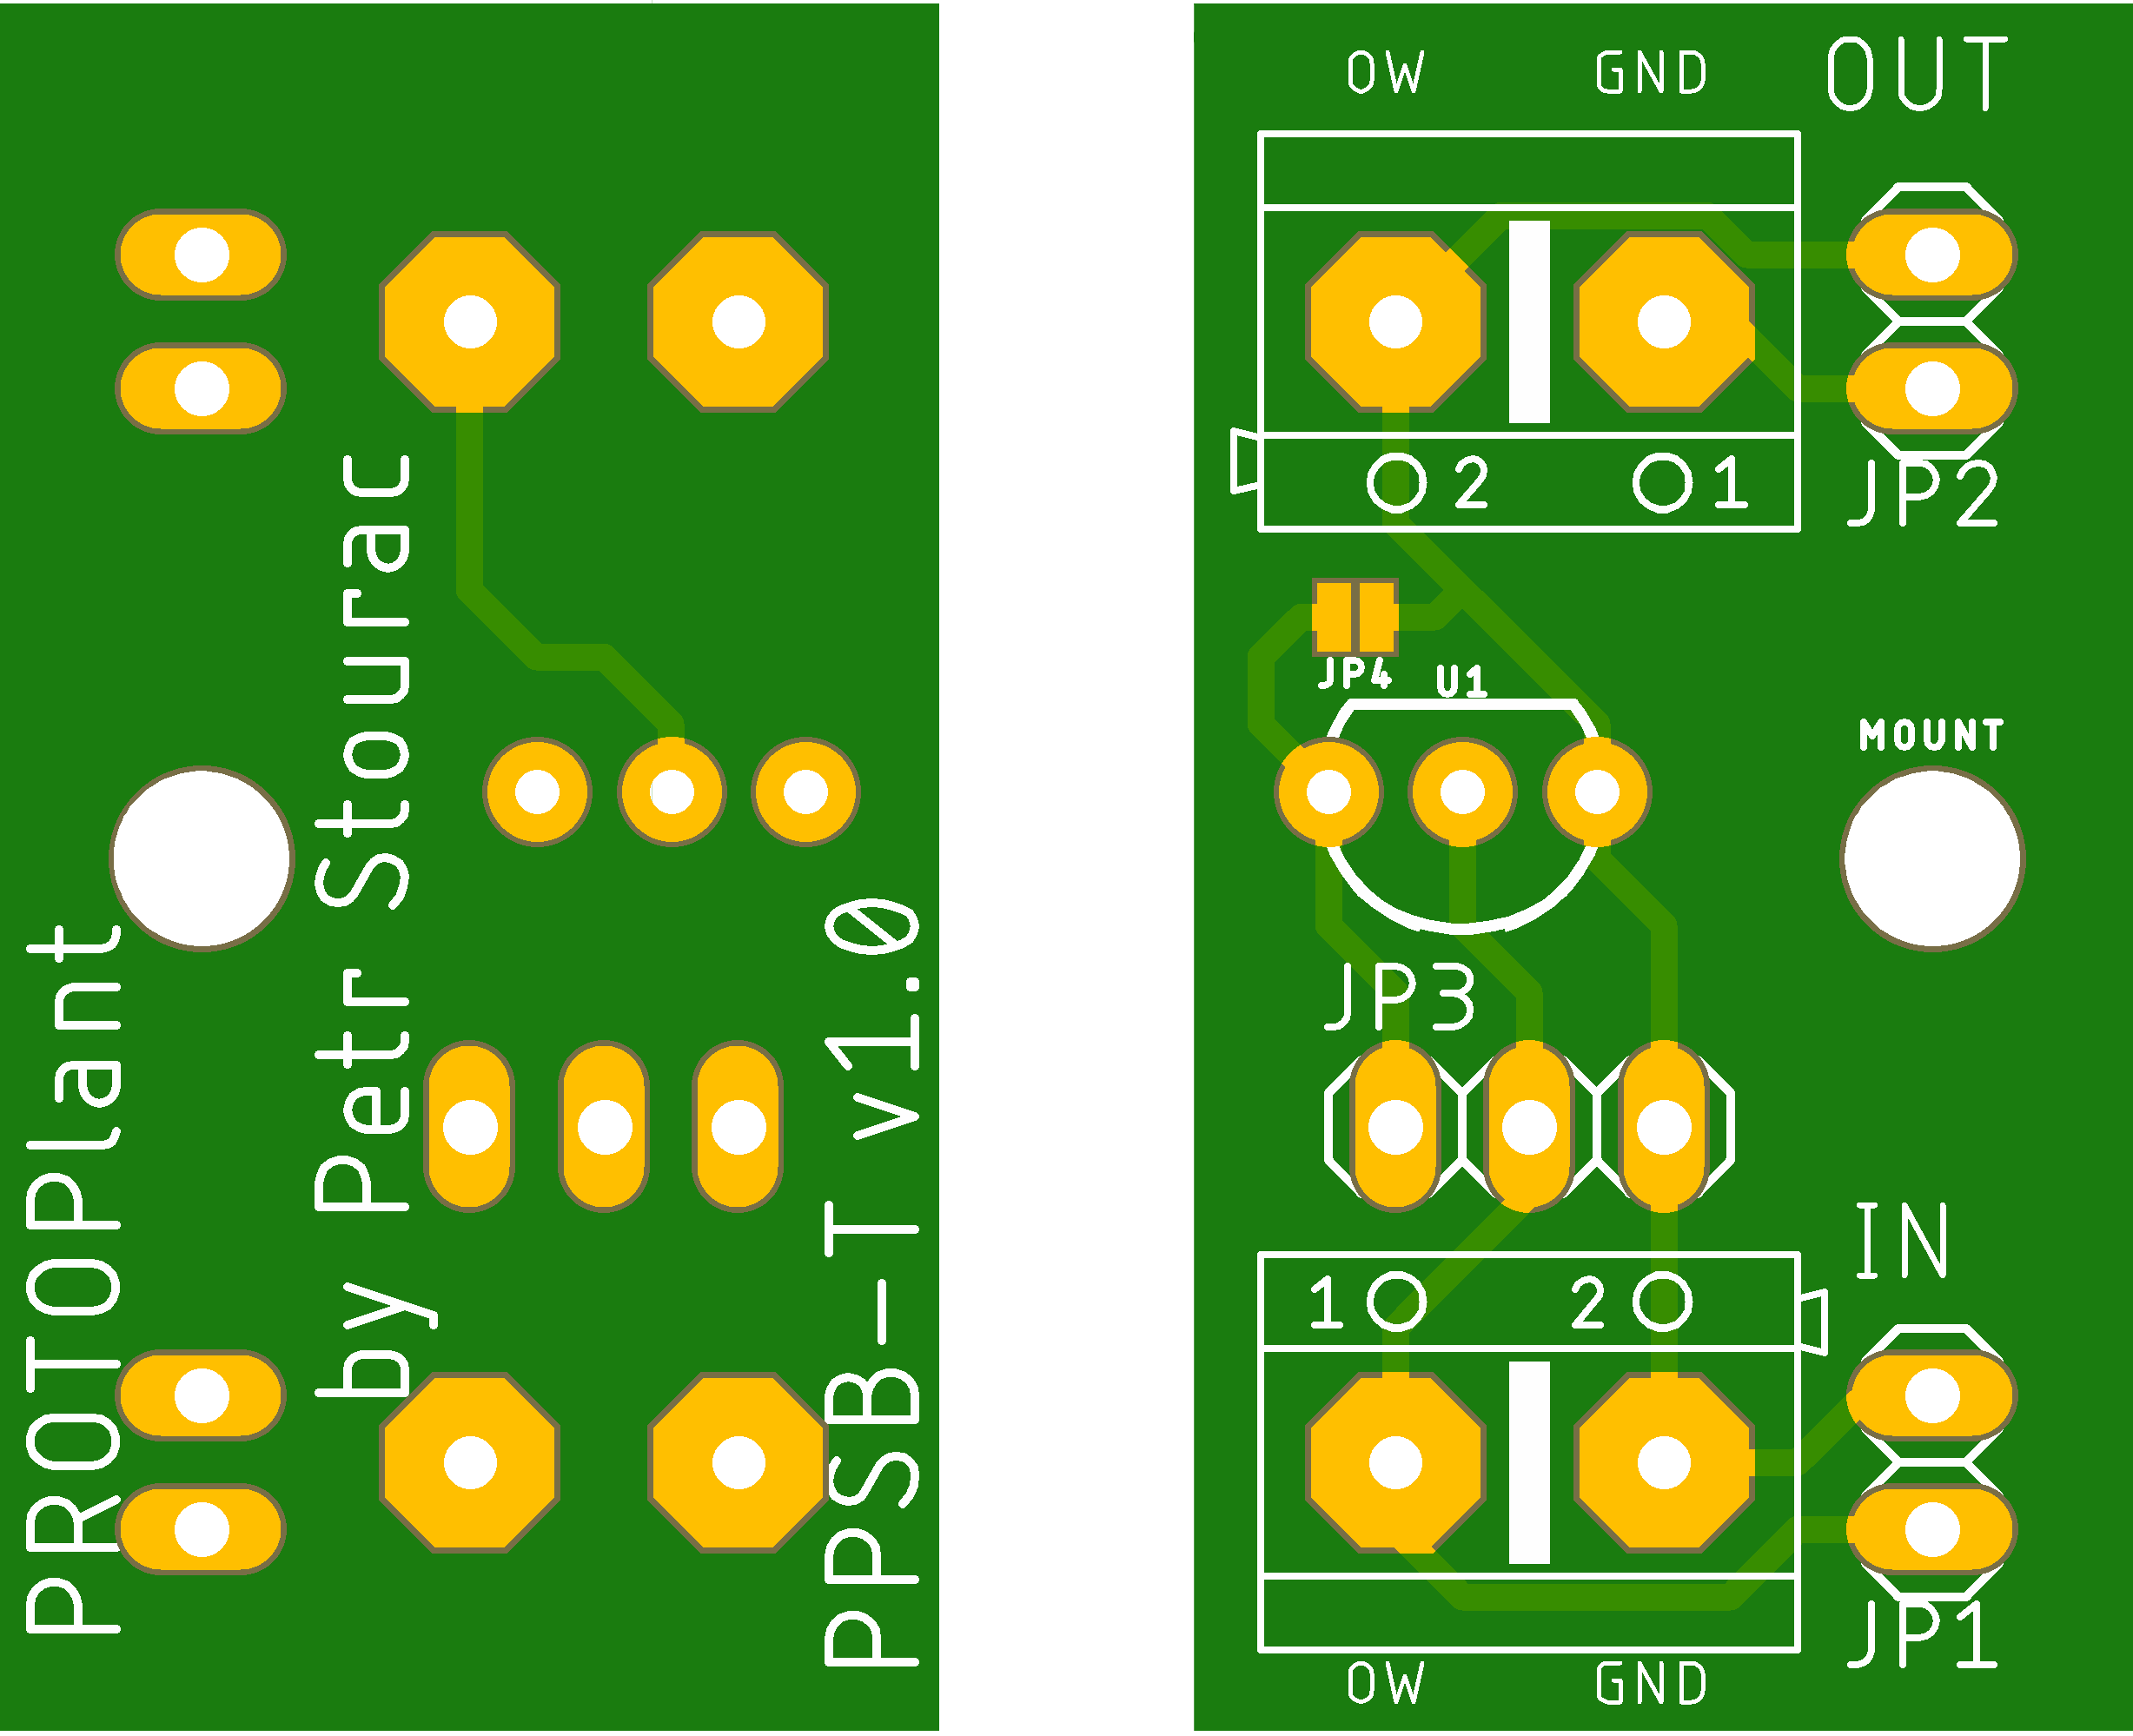
\includegraphics[width=0.85\textwidth]{img/HARDWARE/PPSB-T_BOTH.png}
    \caption{Vizualizace PPSB-T (horní strana vpravo, dolní vlevo).}
    \label{fig:PPSB-T_VISUAL}
\end{figure}

\begin{figure}[h]
    \centering
    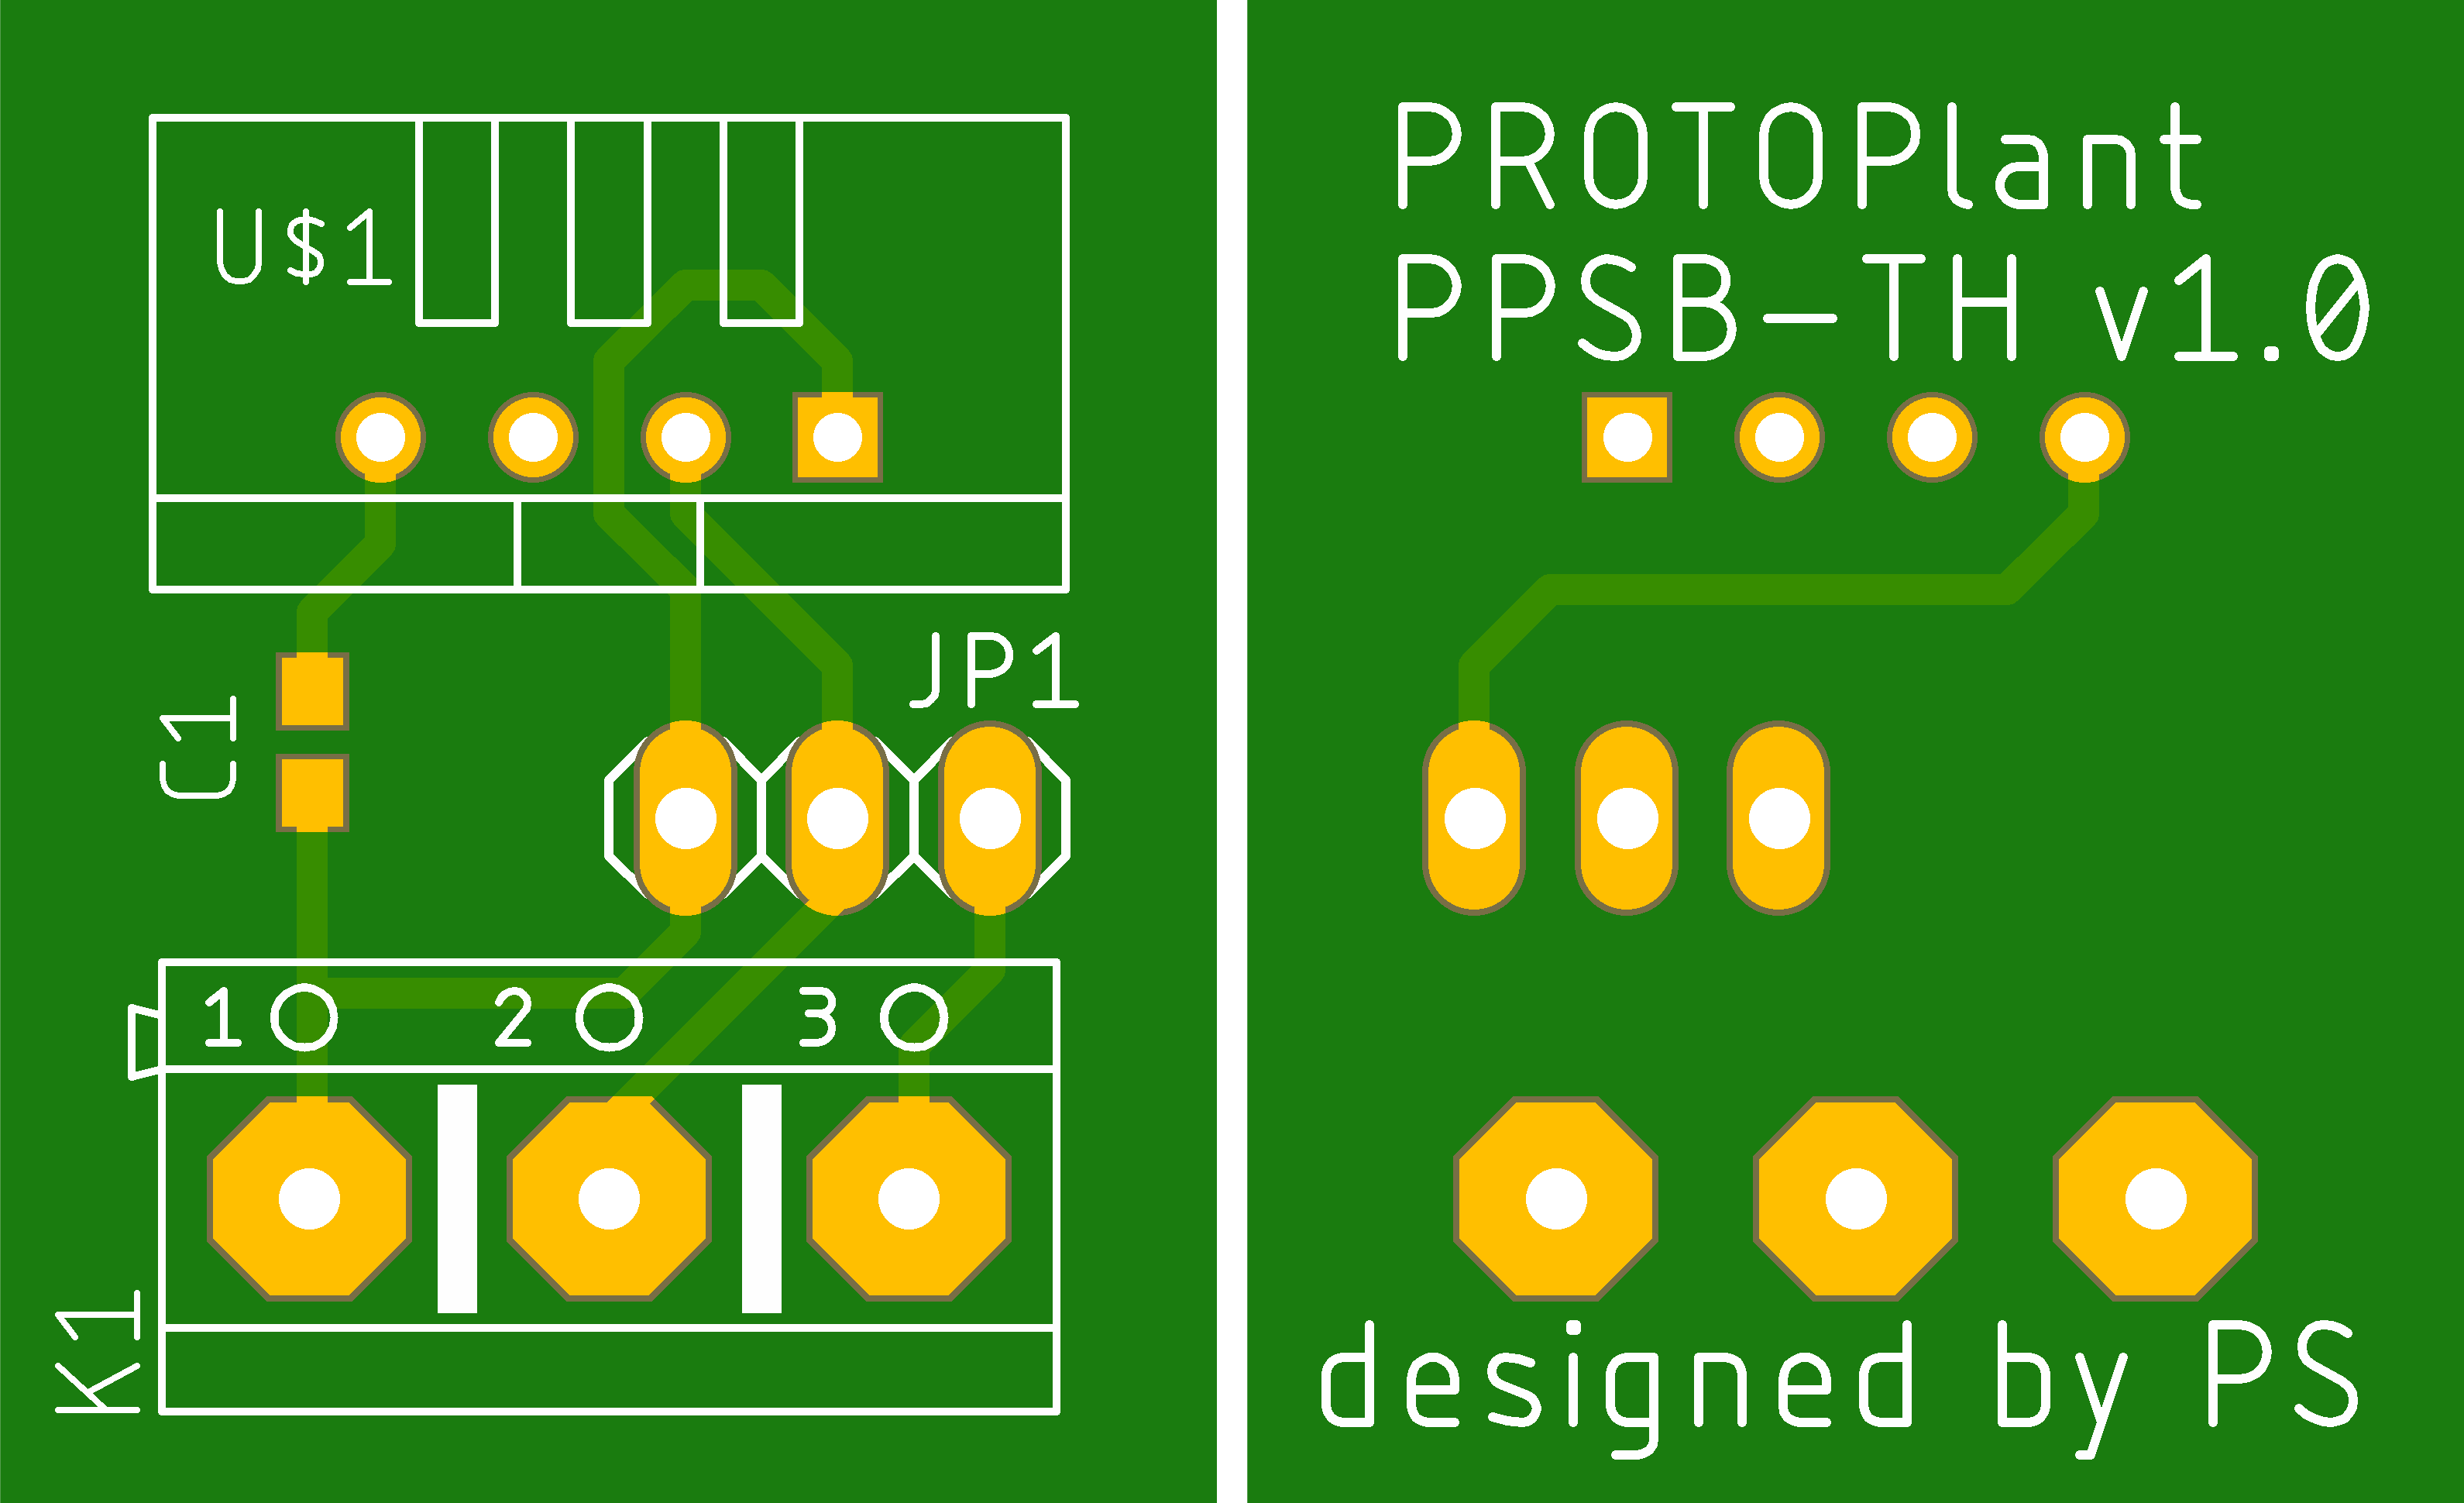
\includegraphics[width=0.85\textwidth]{img/HARDWARE/PPSB-TH_BOTH.png}
    \caption{Vizualizace desky PPSB-TH (horní strana vlevo, dolní vpravo).}
    \label{fig:PPSB-TH_VISUAL}
\end{figure}

\begin{figure}[htbp]
    \centering
    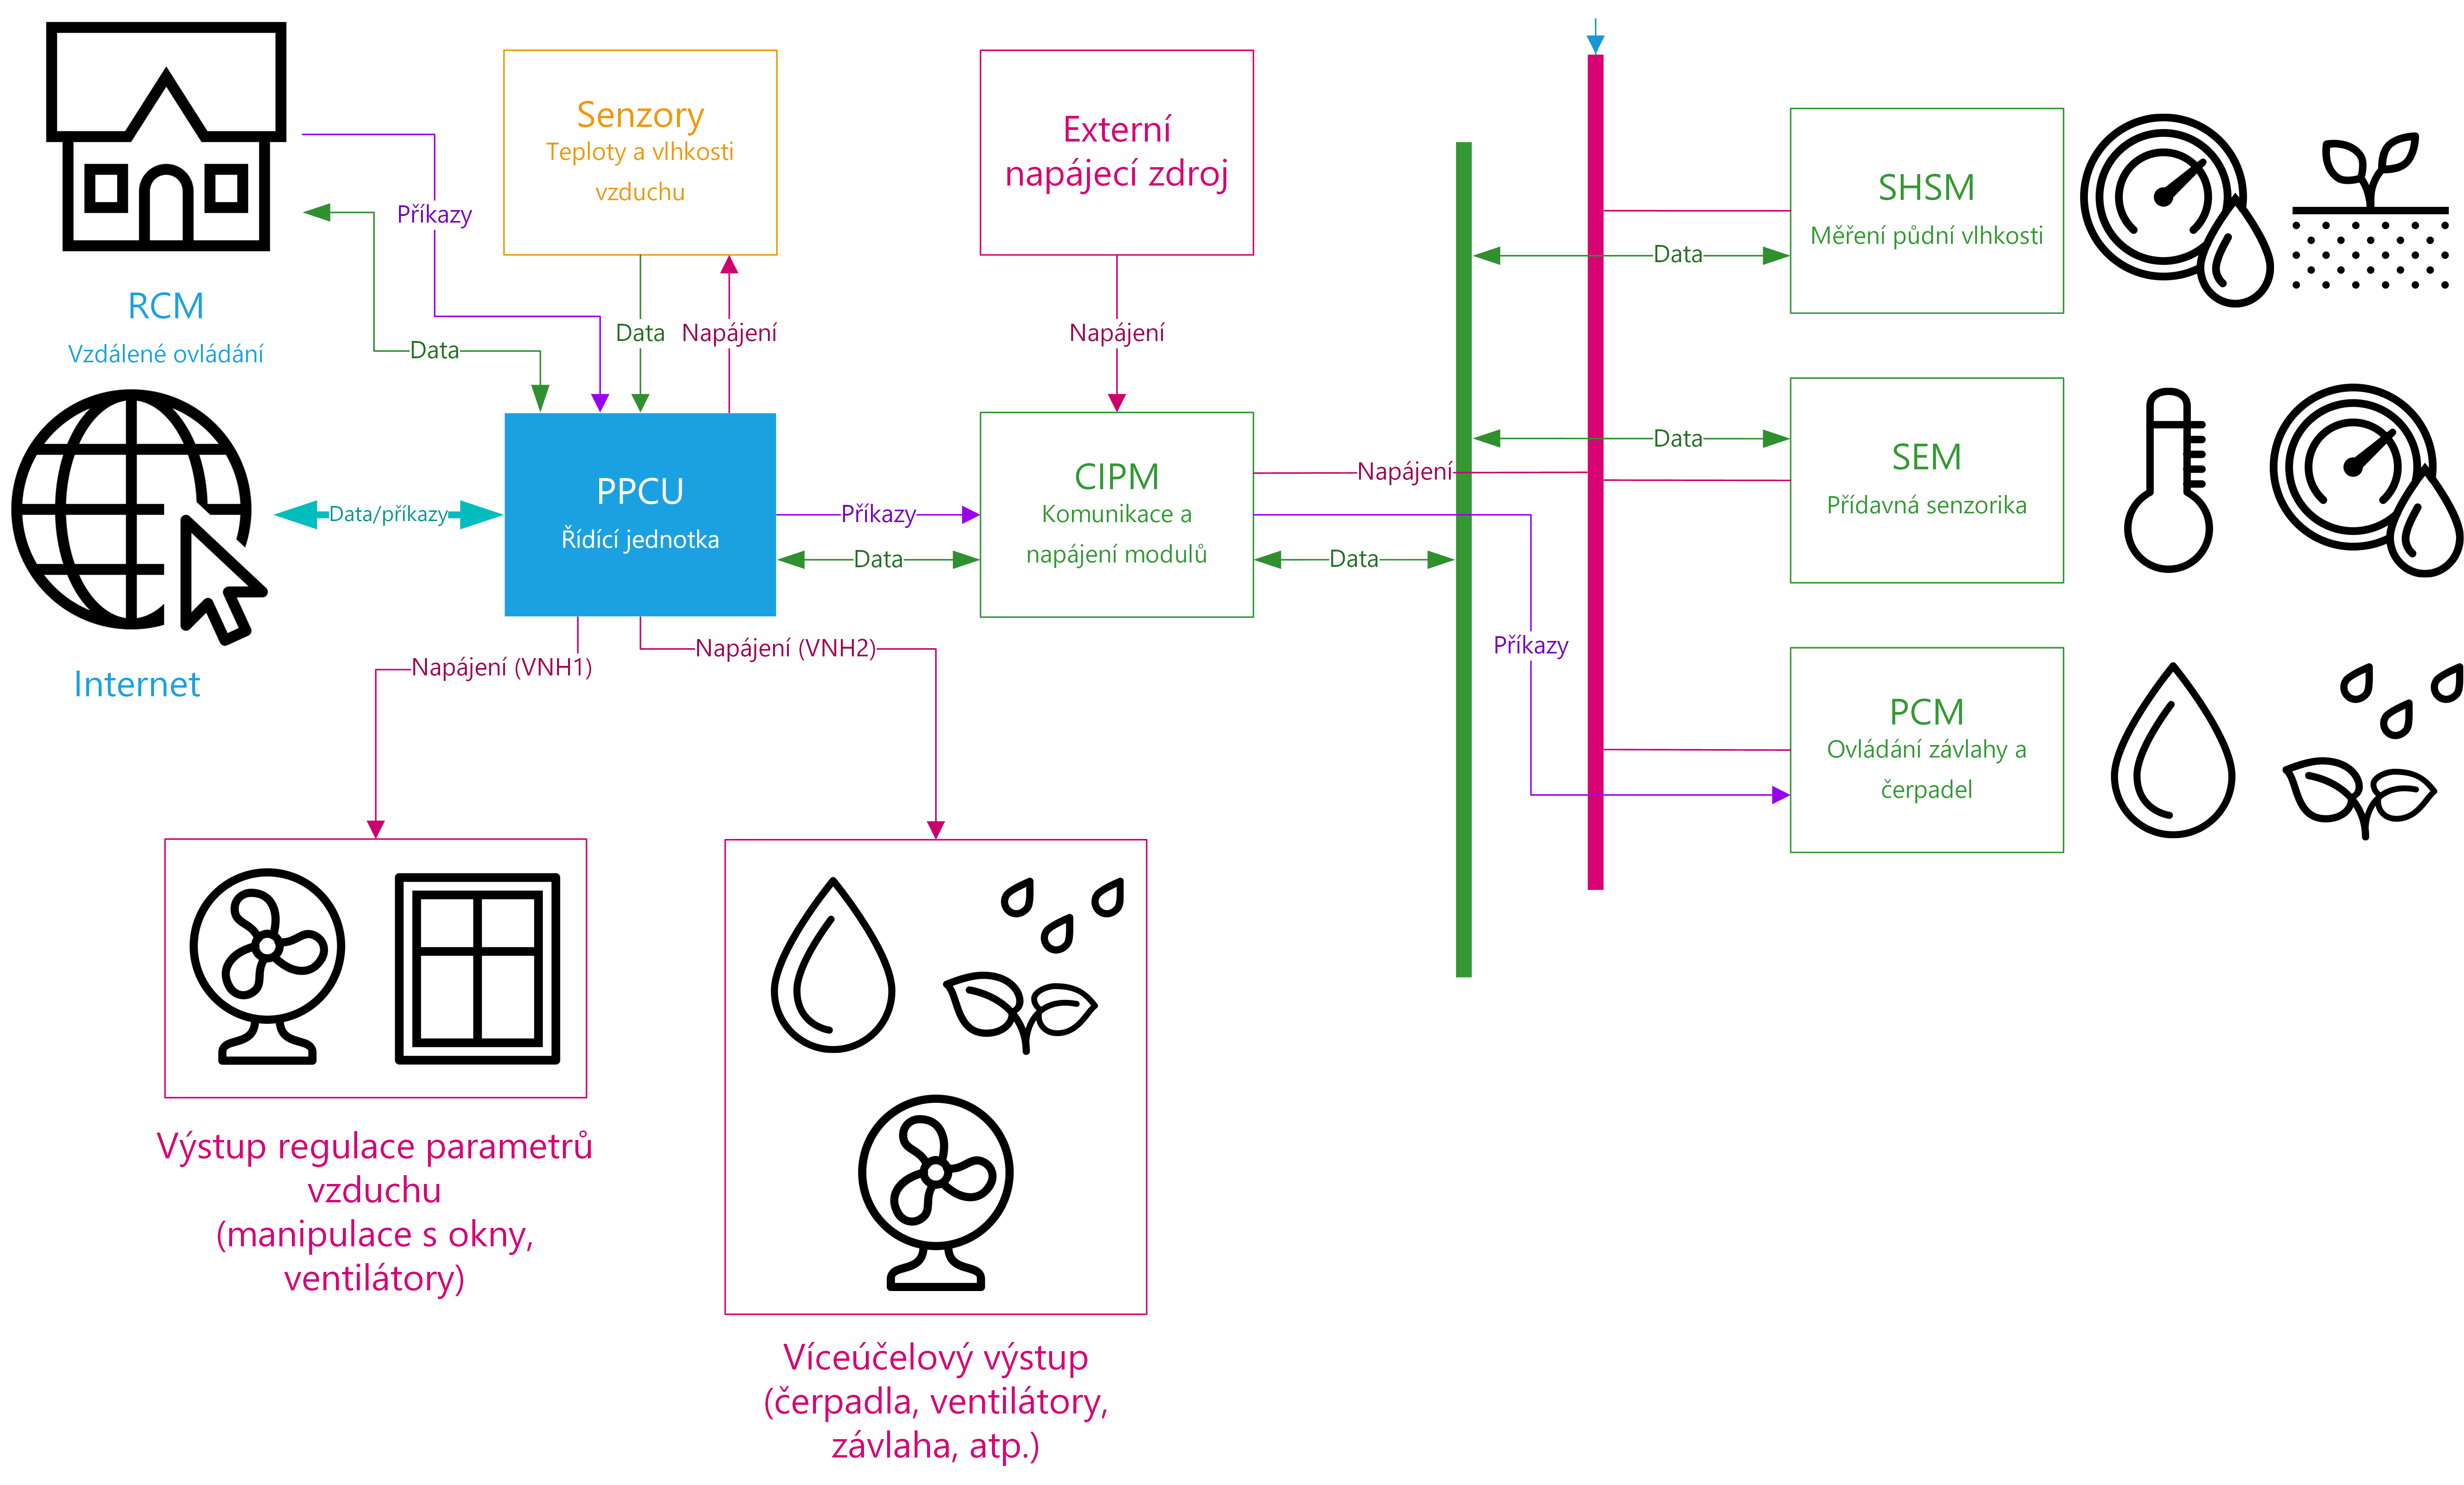
\includegraphics[angle=90,origin=c,scale=0.7]{img/HARDWARE/MODULES.png}
    \caption{Schéma zapojení a~funkce jednotlivých modulů.}
    \label{fig:add-MODULES}
 \end{figure}

\begin{figure}[h]
    \centering
    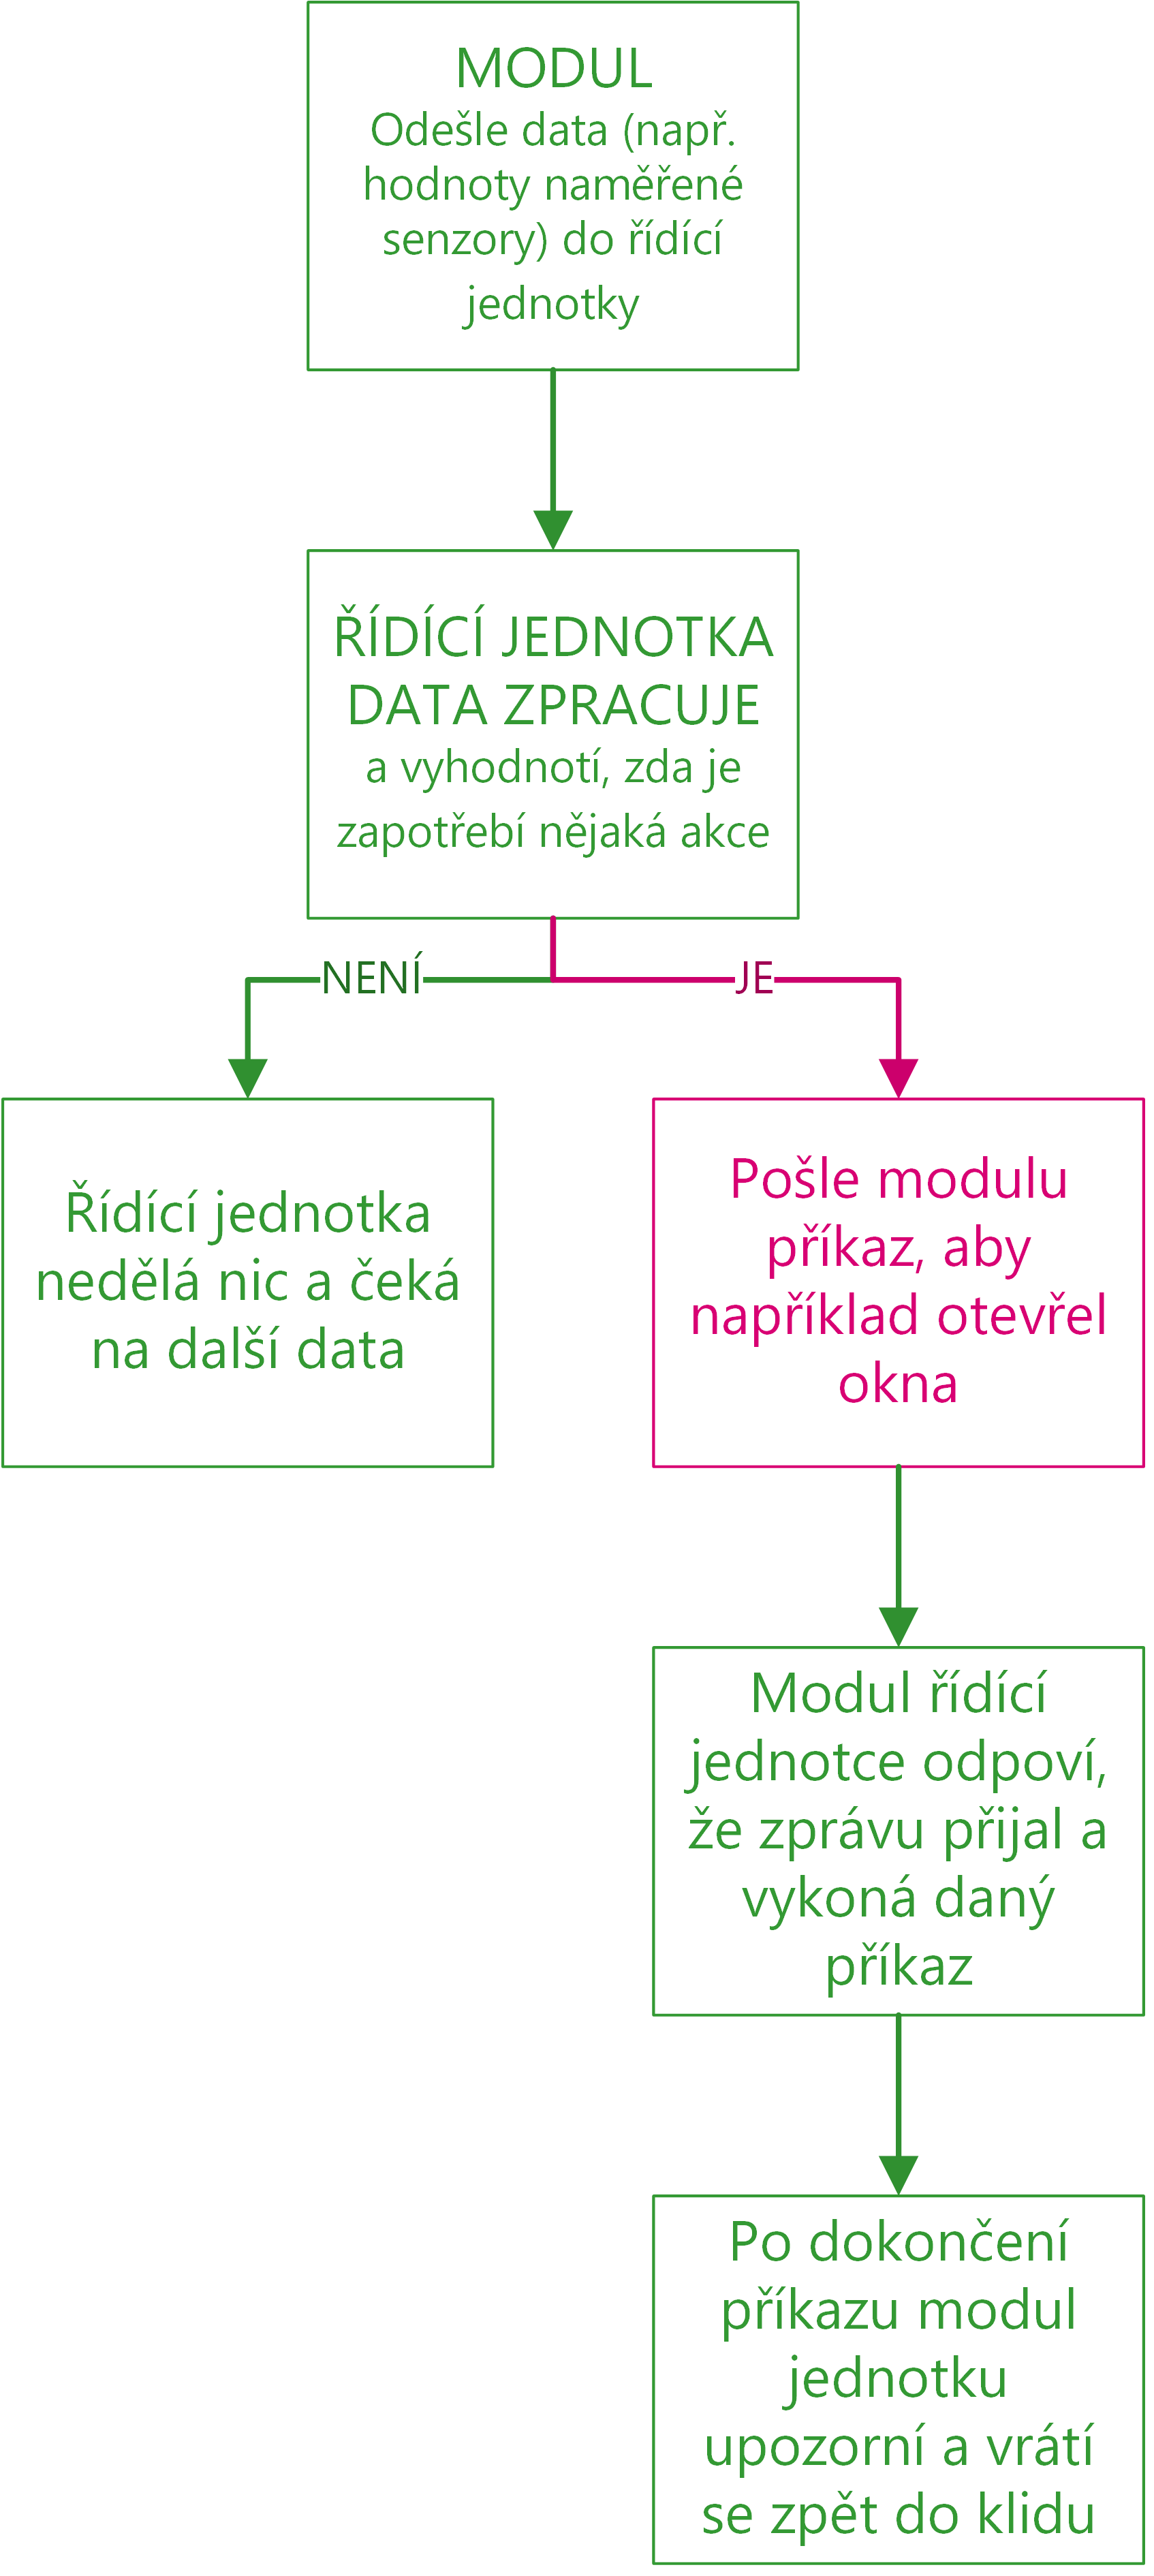
\includegraphics[scale=0.9]{img/SOFTWARE/KOMUNIKACE_MODULU.png}
    \caption{Blokový diagram komunikace řídící jednotky a~přídavného modulu.}
    \label{fig:PPCU-to-MODULE-communication}
\end{figure}

\begin{figure}[htbp]
    \centering
    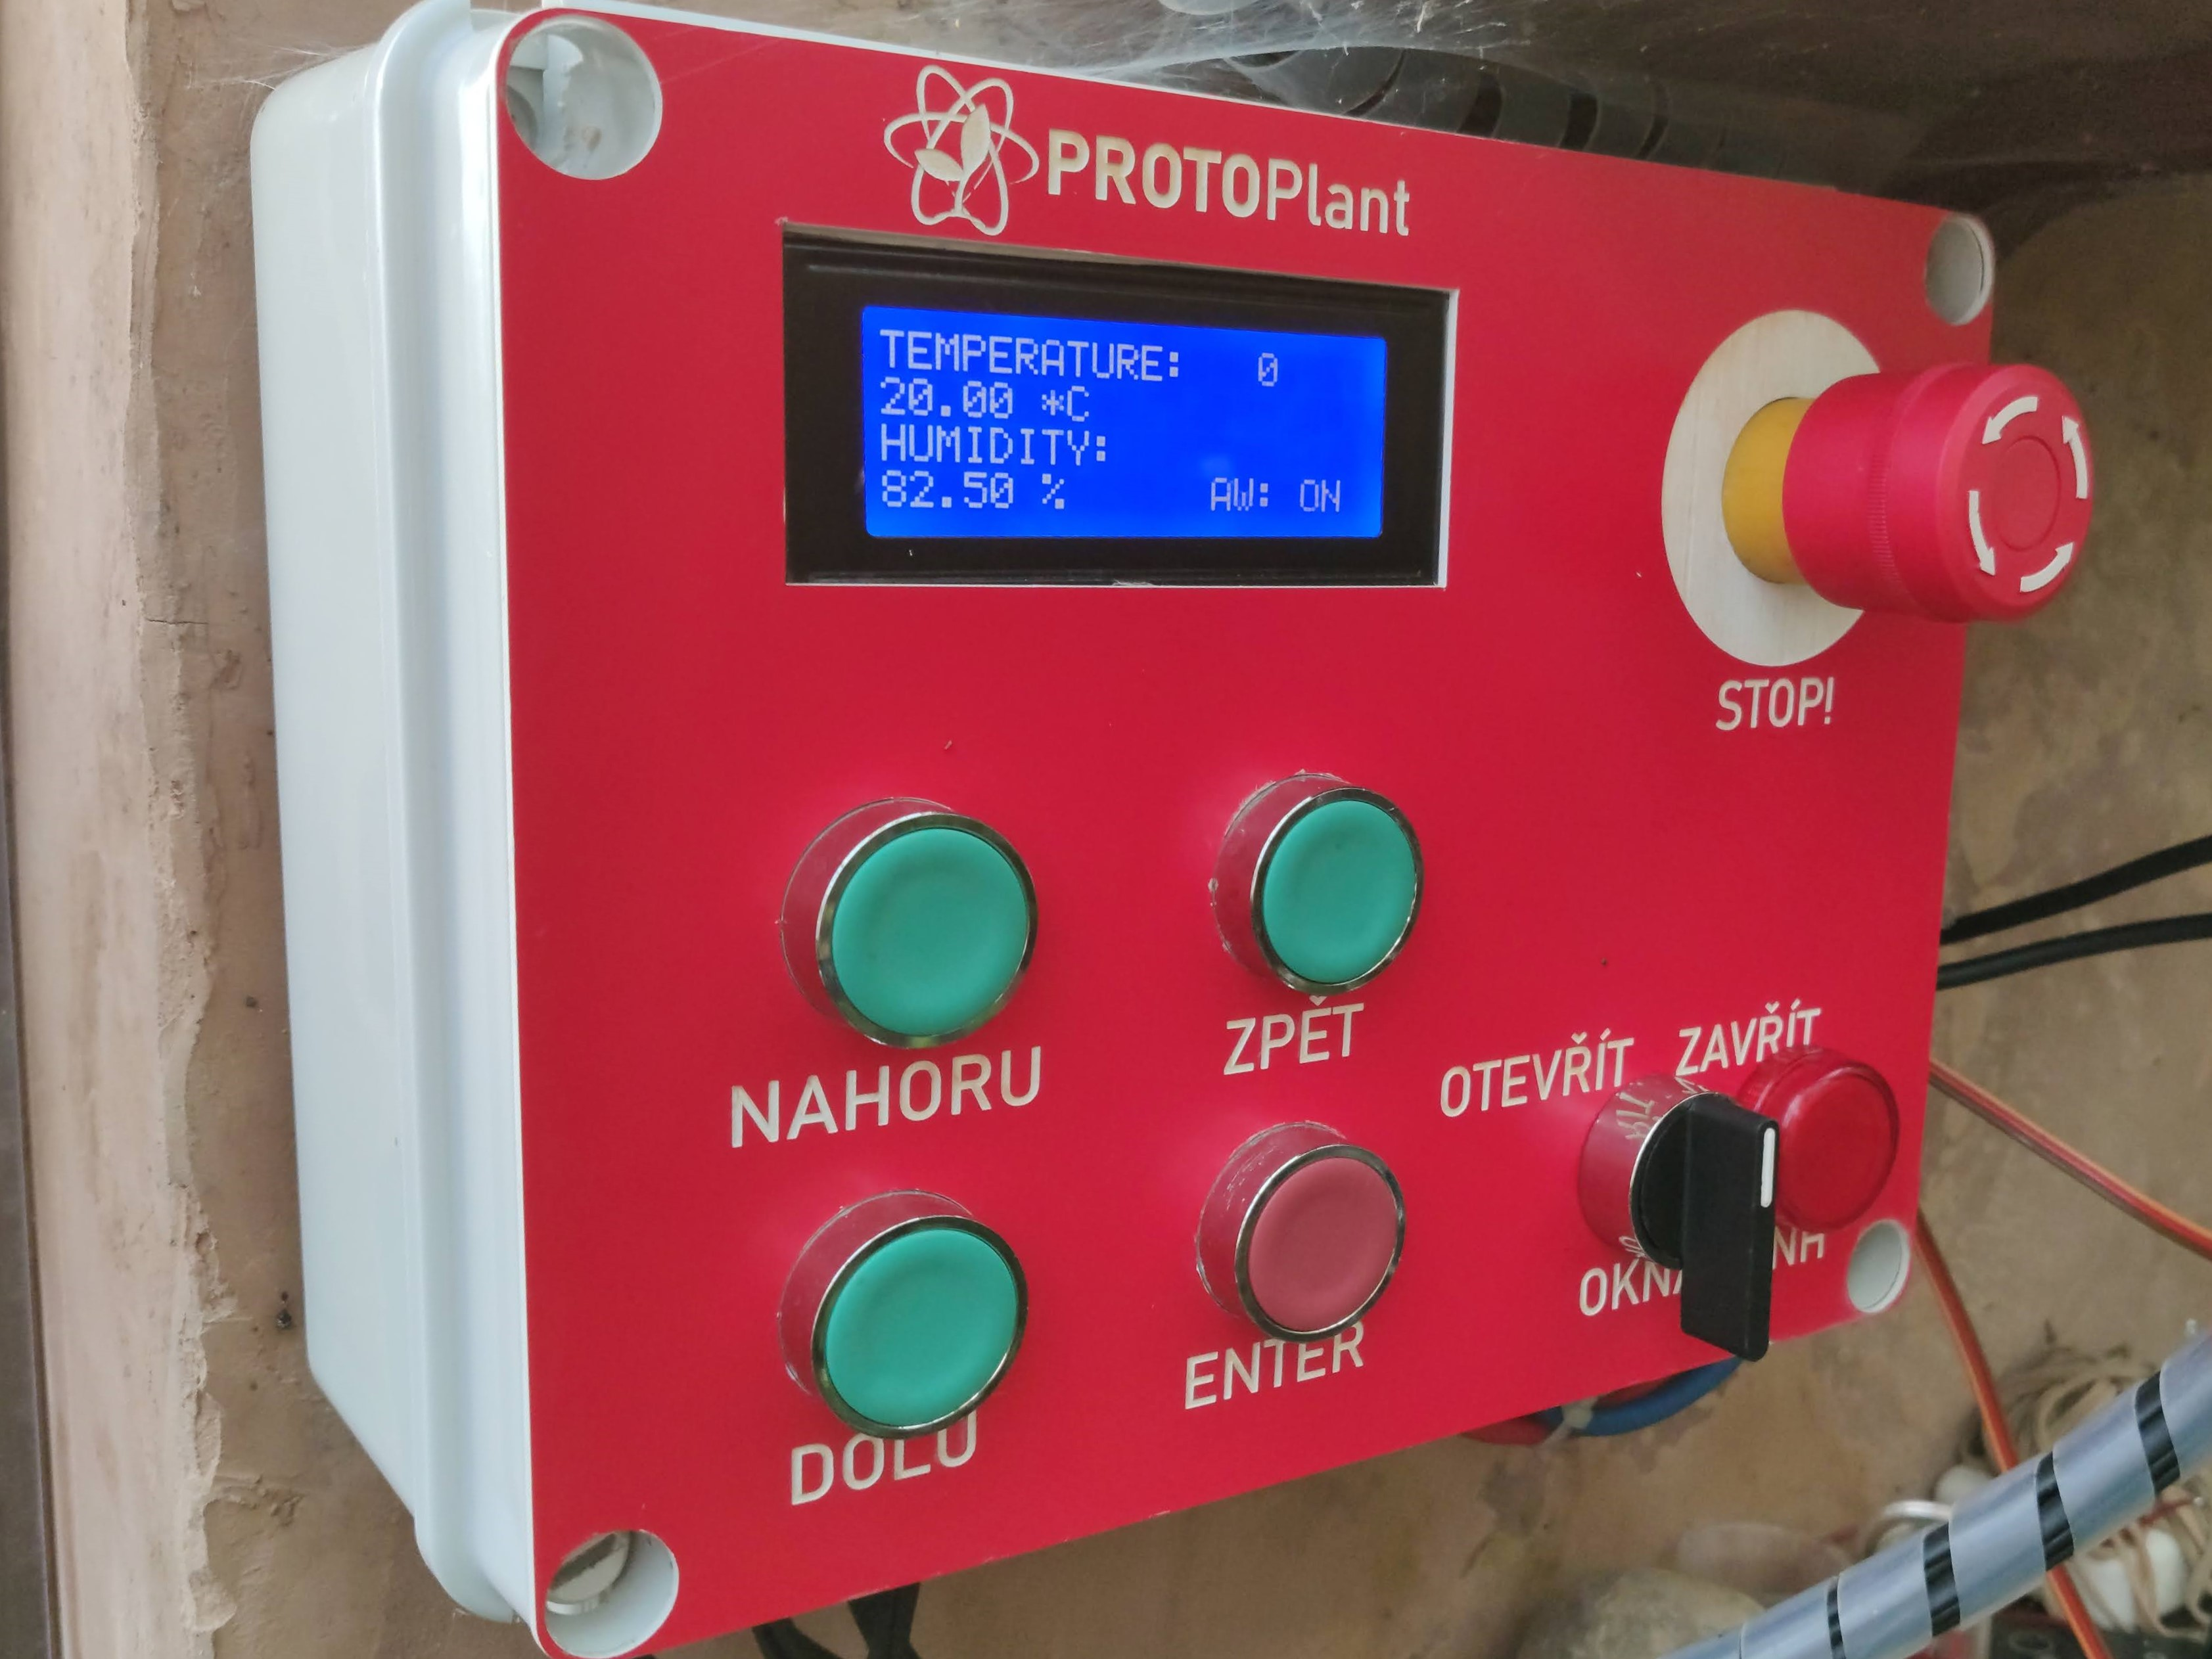
\includegraphics[width=0.85\textwidth]{img/PHOTOS/ControlUnit1.jpg}
    \caption{Fotografie řídící jednotky instalované v~testovacím skleníku (verze 4.9).}
    \label{fig:PPCU1}
\end{figure}

\begin{figure}[htbp]
    \centering
    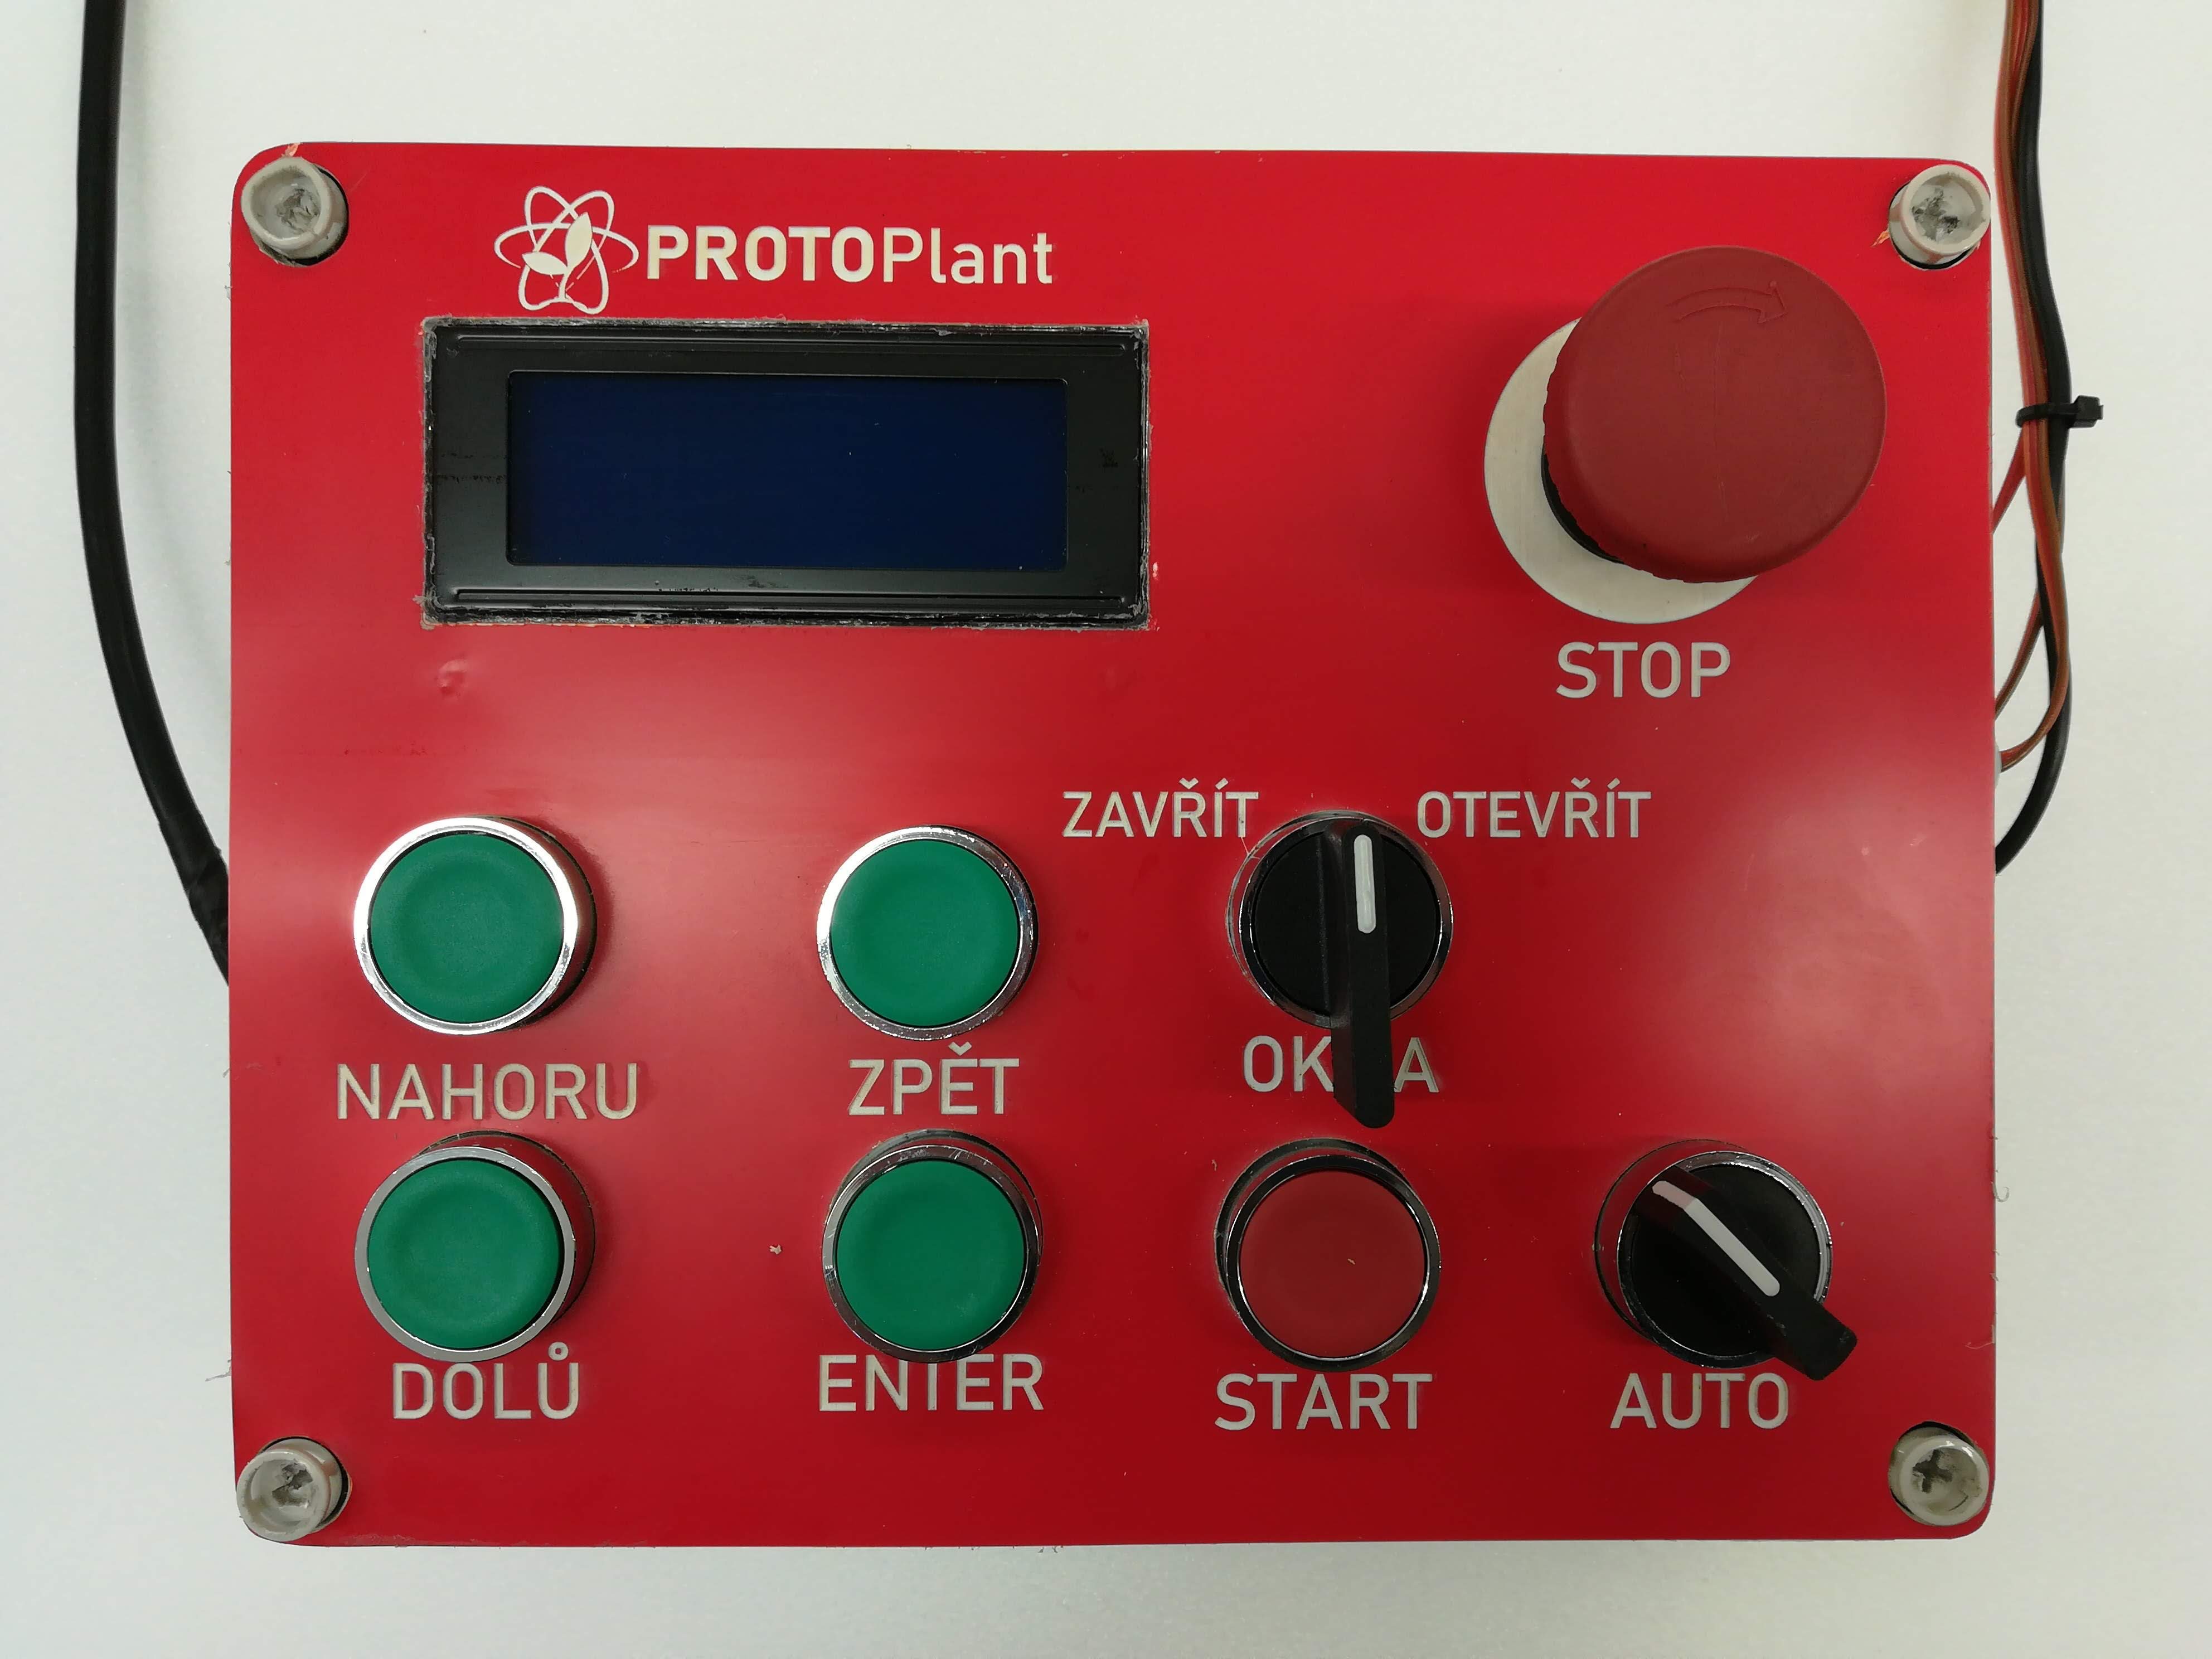
\includegraphics[width=0.85\textwidth]{img/PHOTOS/ControlUnit2.jpg}
    \caption{Fotografie prototypu řídící jednotky verze 3.1.}
    \label{fig:PPCU2}
\end{figure}

\begin{figure}[htbp]
    \centering
    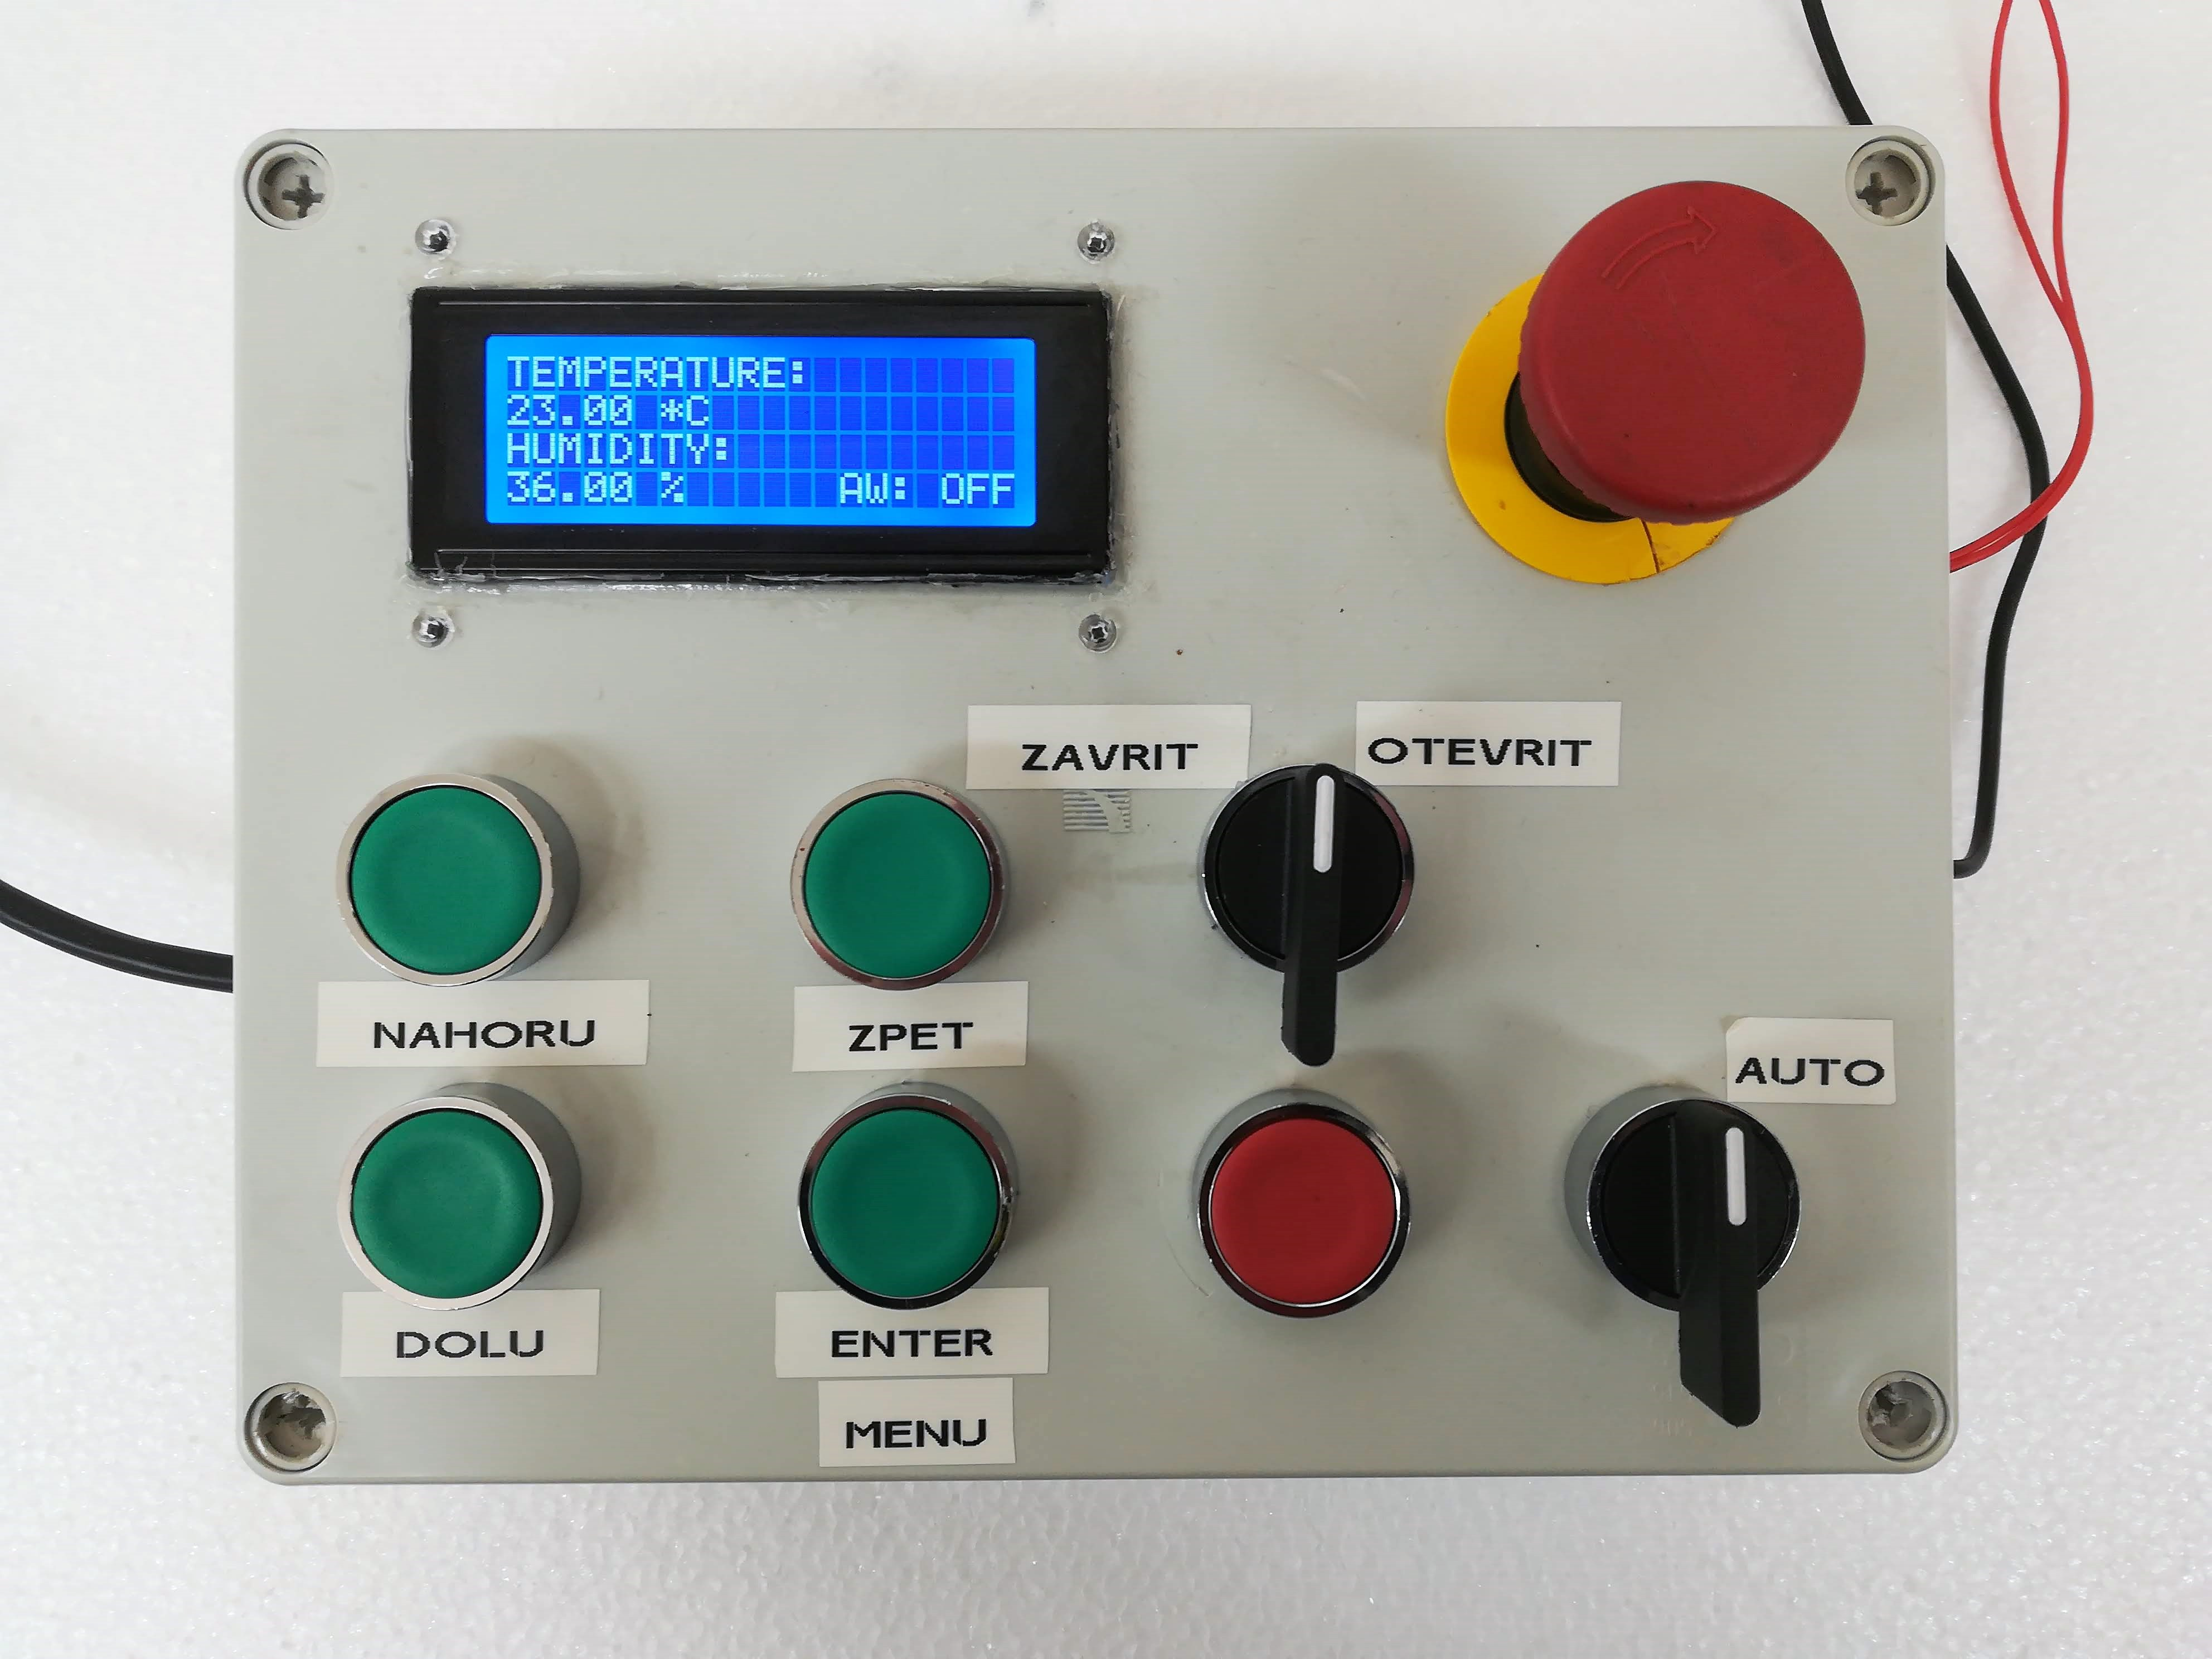
\includegraphics[width=0.85\textwidth]{img/PHOTOS/ControlUnitOLD.jpg}
    \caption{Fotografie prototypu řídící jednotky verze 3.0.}
    \label{fig:PPCU_v3_0}
\end{figure}

\begin{figure}[htbp]
    \centering
    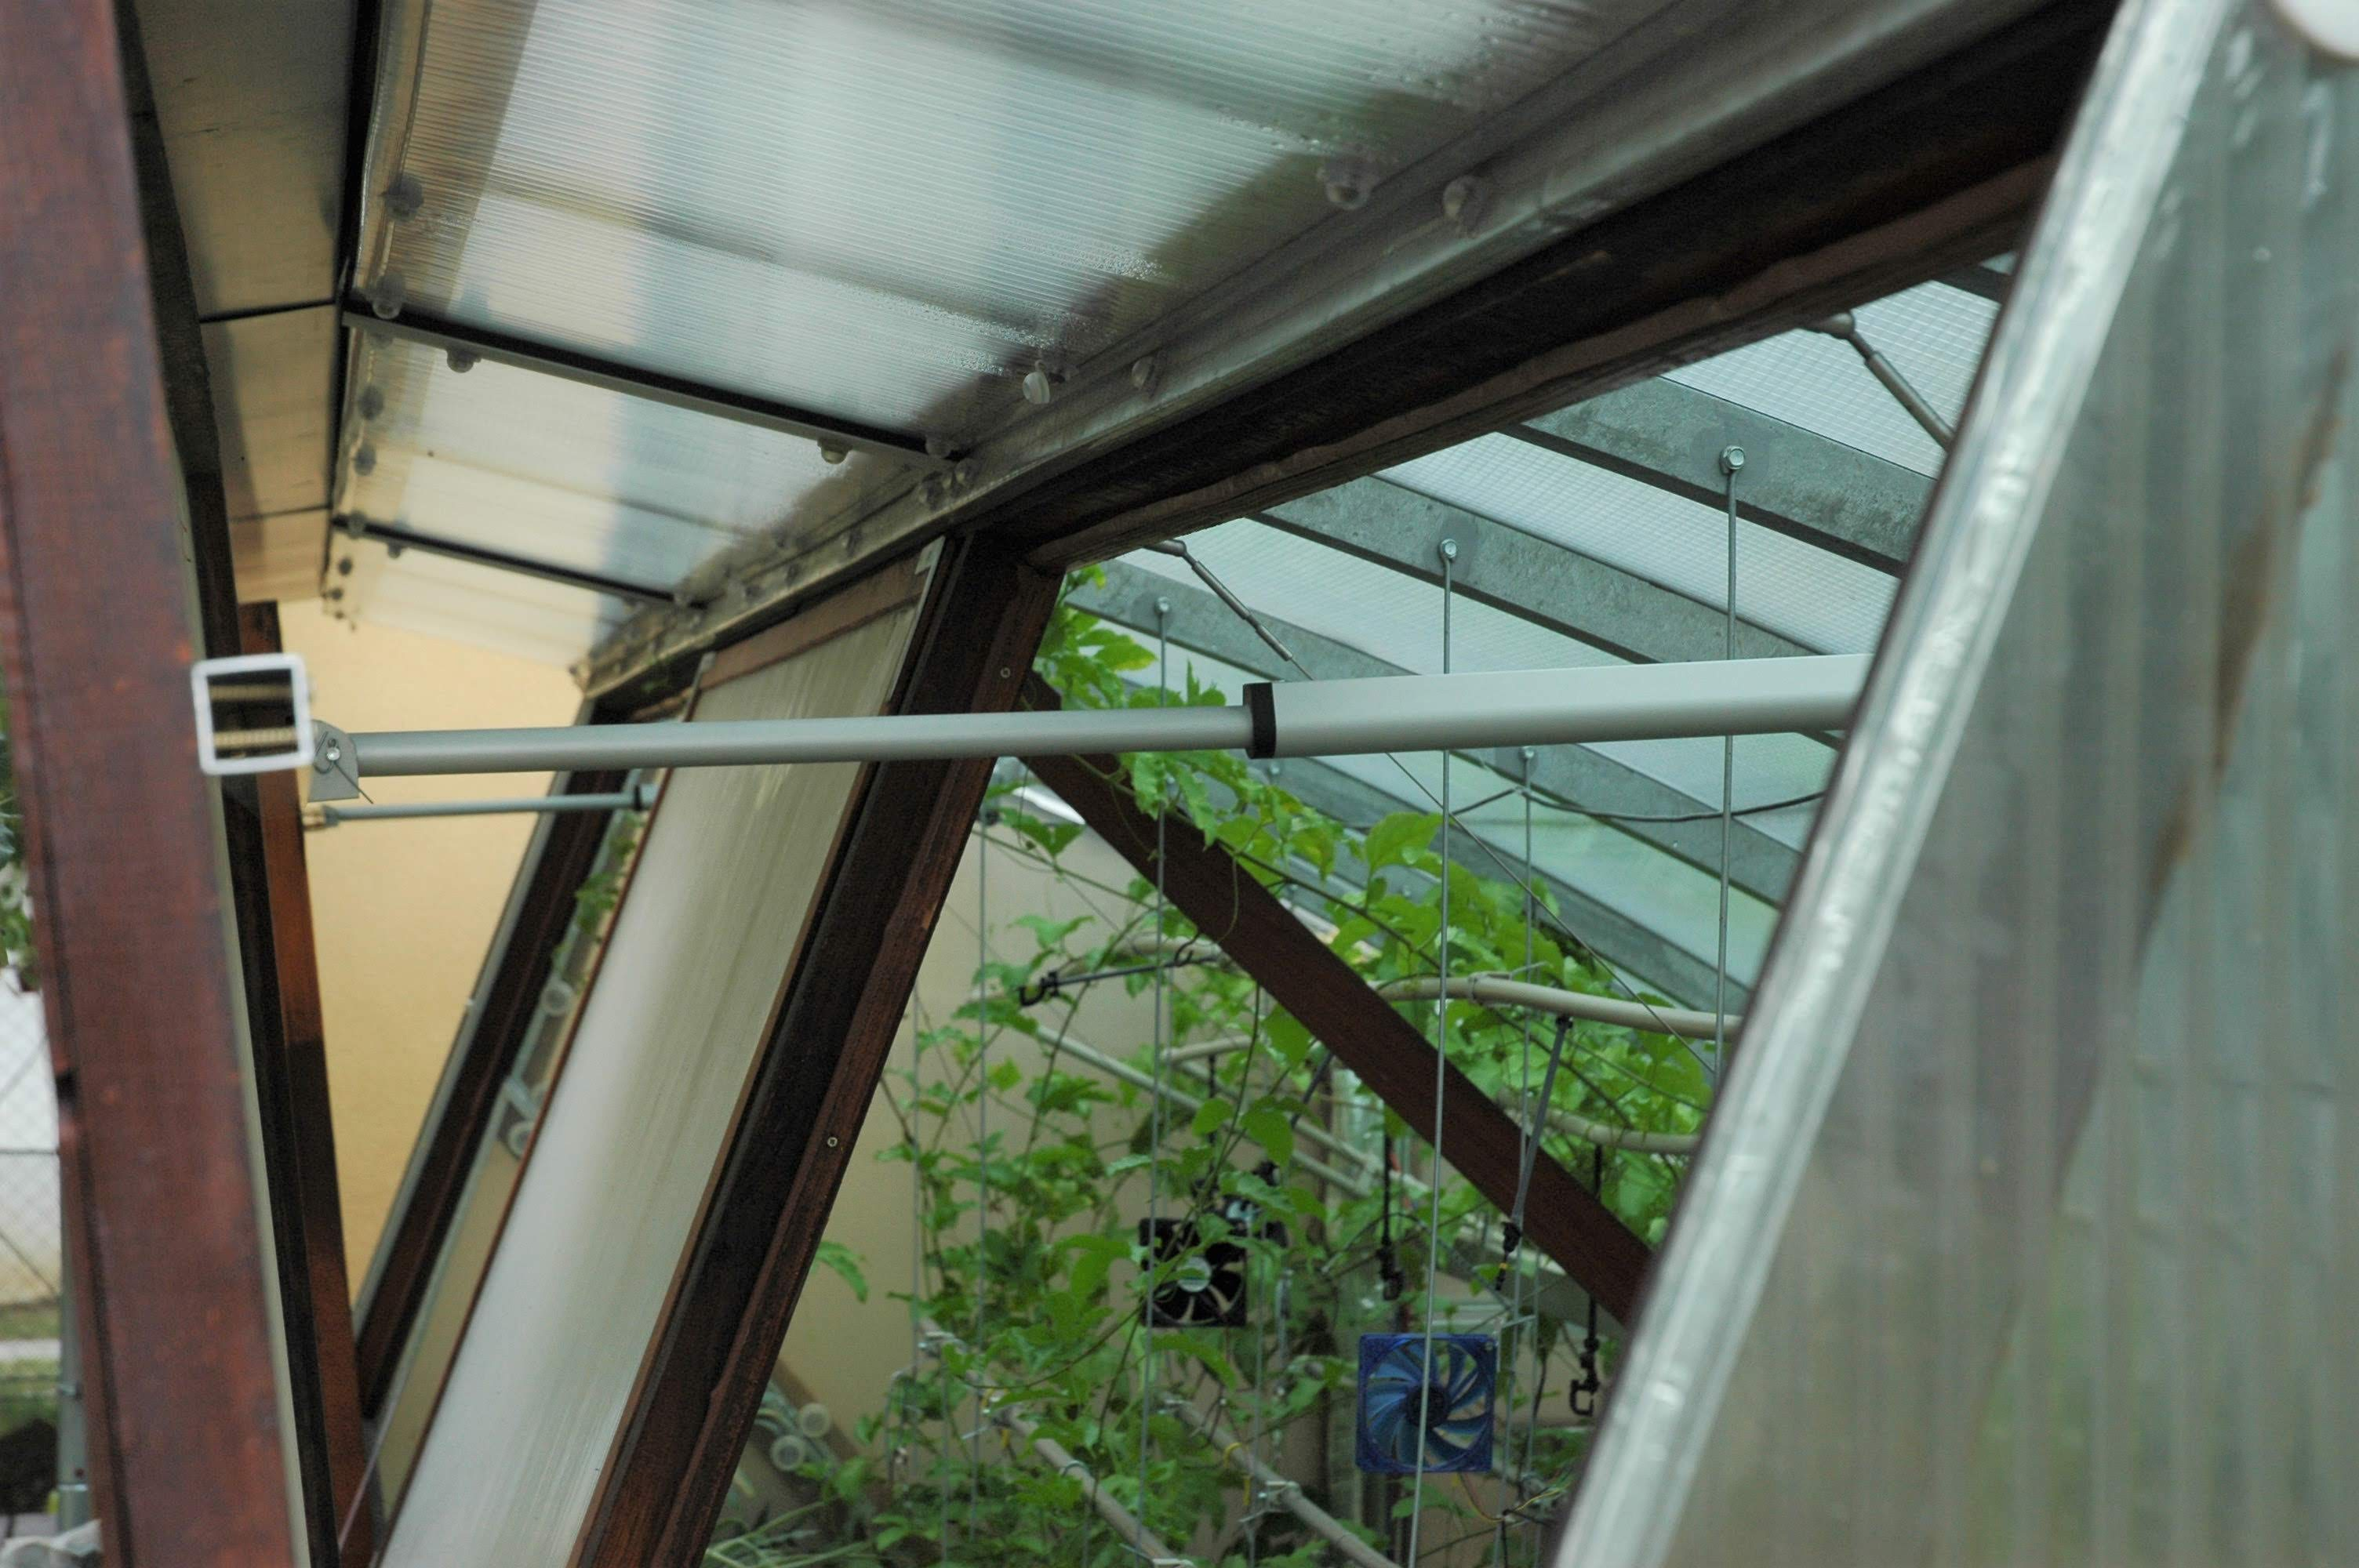
\includegraphics[width=0.85\textwidth]{img/PHOTOS/VS_1.jpg}
    \caption{Fotografie otevřeného okna testovacího skleníku.}
    \label{fig:OPEN_WINDOW}
\end{figure}

\begin{figure}[htbp]
    \centering
    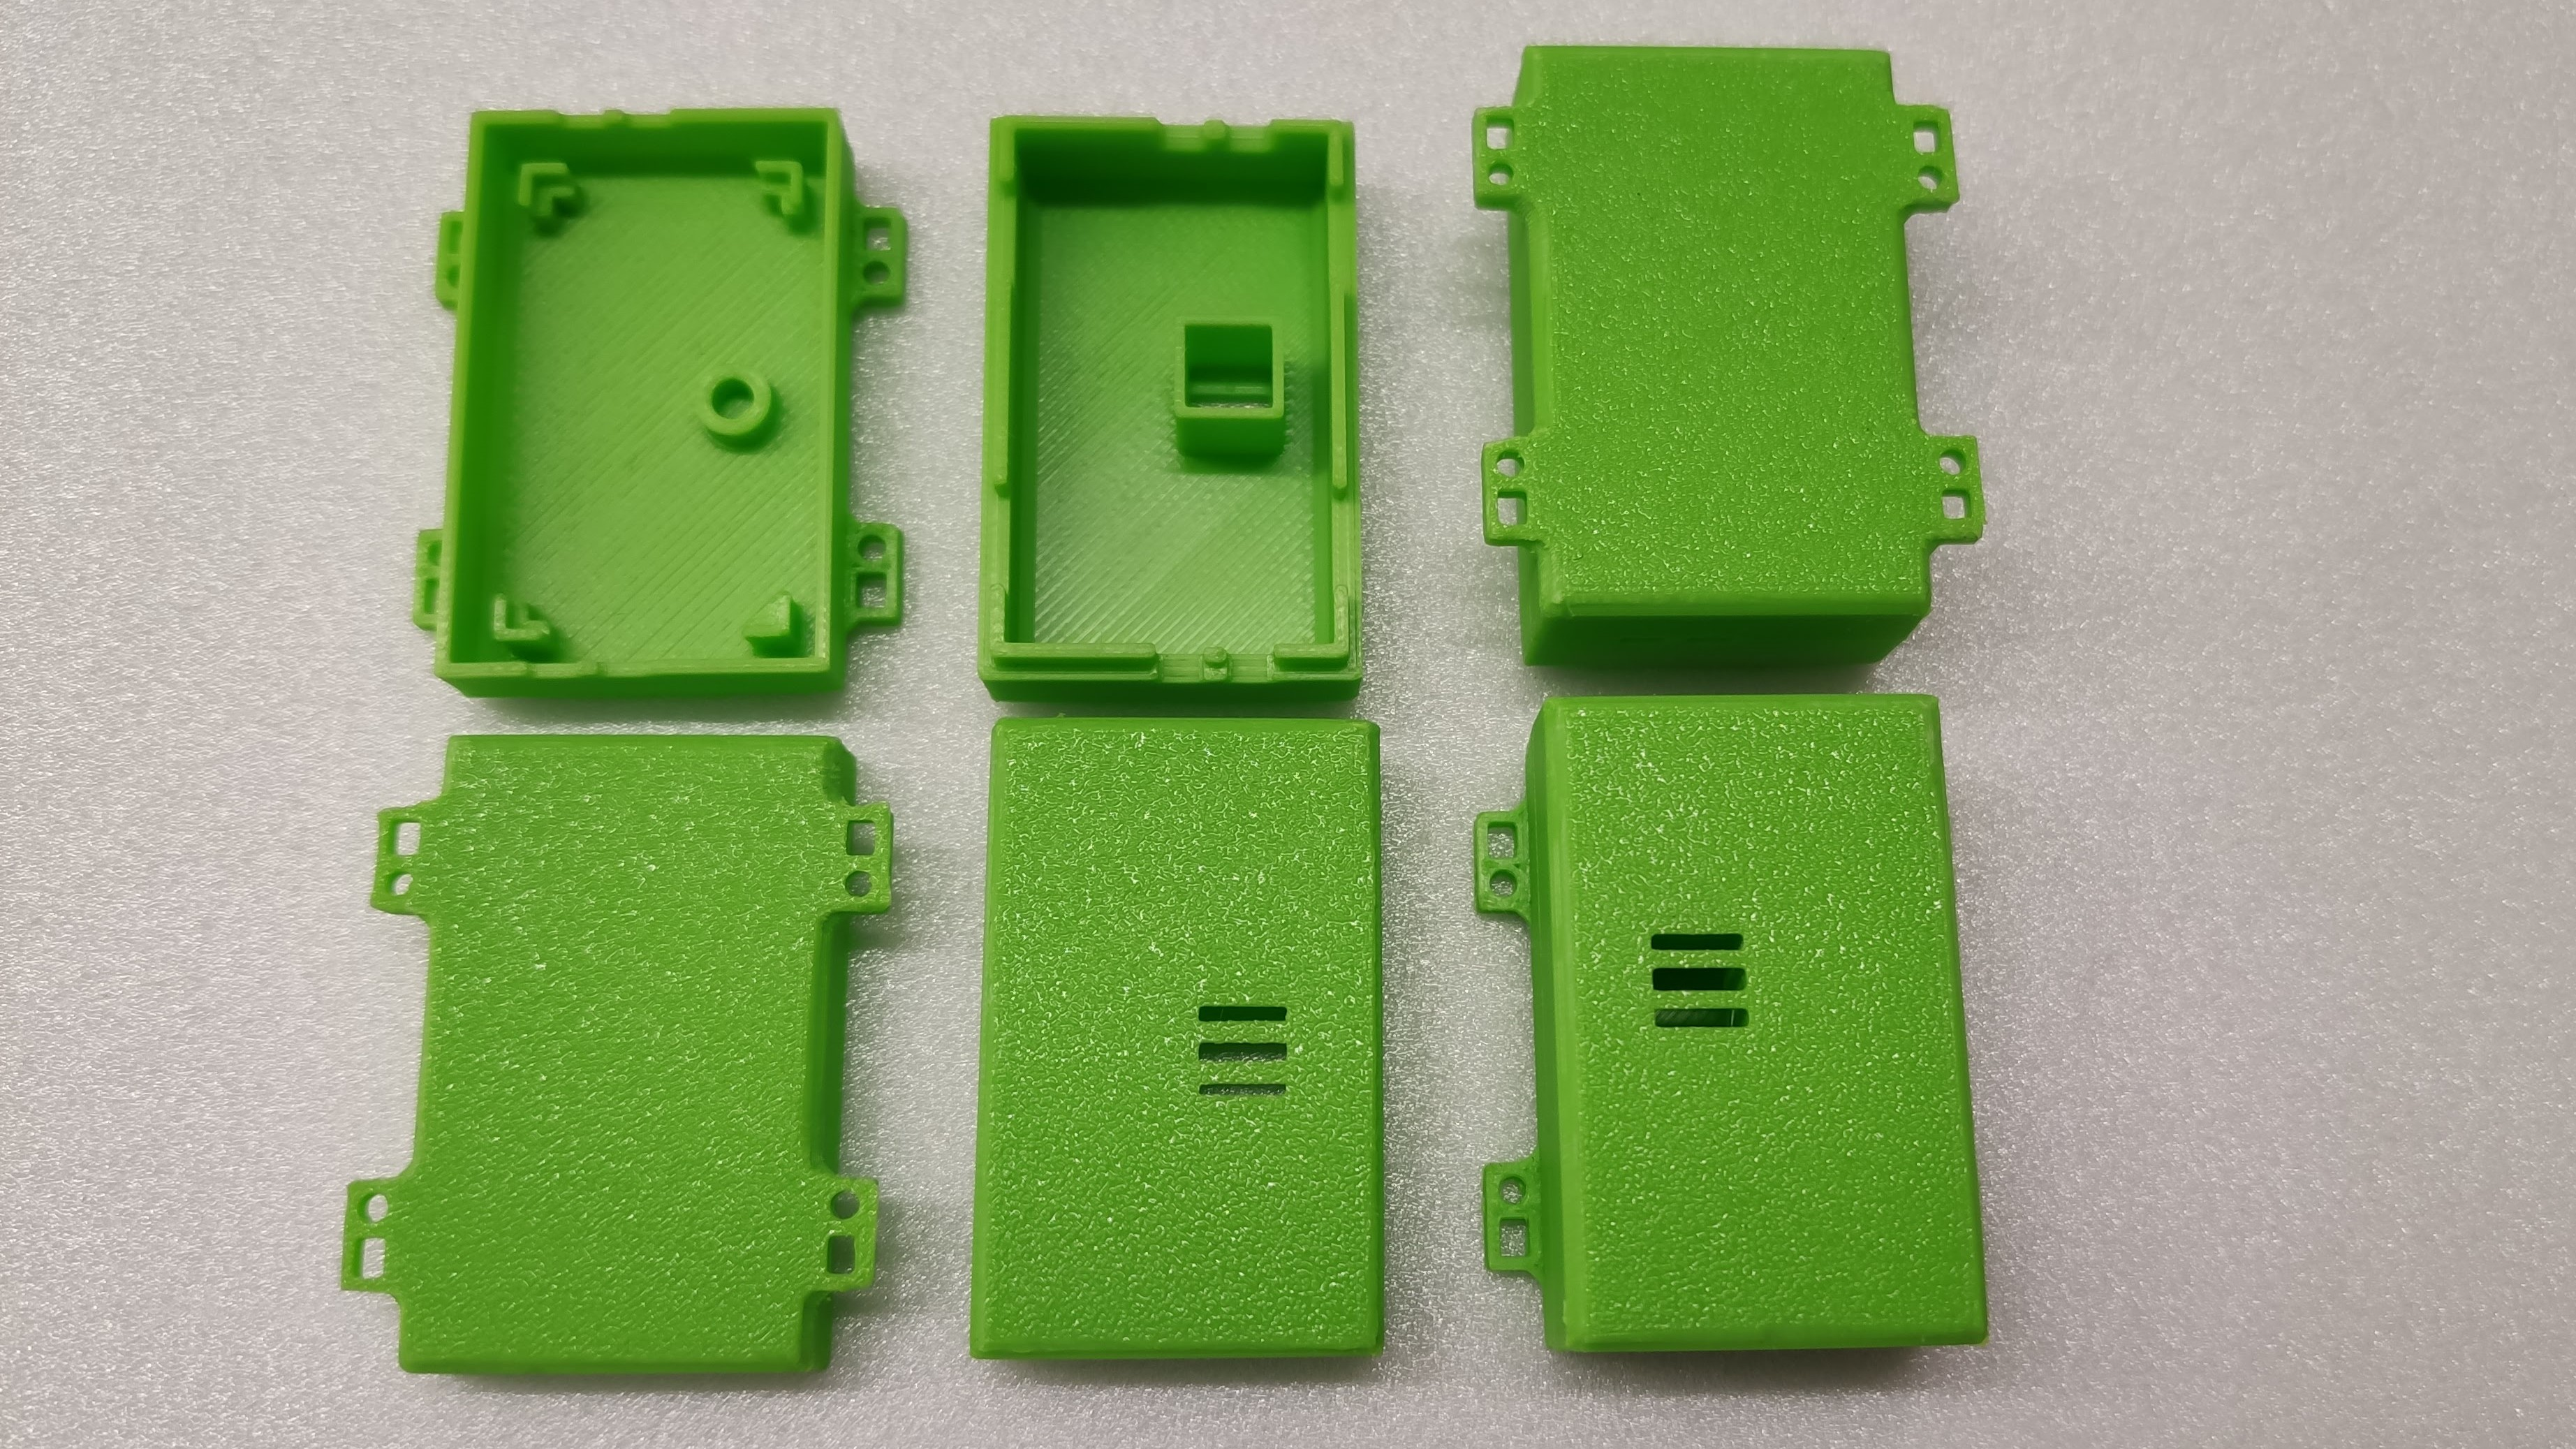
\includegraphics[width=\textwidth]{img/PHOTOS/PPSB-T_cases.jpg}
    \caption{Krabičky na desky PPSB.}
    \label{fig:PPSB-T_cases}
\end{figure}

\newpage

\printbibliography[title=Literatura]
\addcontentsline{toc}{chapter}{Literatura}

\listoffigures
\addcontentsline{toc}{section}{Seznam obrázků}

\listoftables
\addcontentsline{toc}{section}{Seznam tabulek}

\end{document}
